\documentclass[11pt]{report}

\usepackage[utf8]{inputenc}
\usepackage[super]{nth}
\usepackage{graphicx}
\usepackage{comment}

\usepackage{titlesec}
\titleformat{\chapter}[display]   
{\normalfont\huge\bfseries}{\chaptertitlename\ \thechapter}{20pt}{\Huge}   
\titlespacing*{\chapter}{0pt}{-50pt}{40pt}

\begin{document}

\begin{center}
\vspace*{\fill}
This document presents historical events known to mankind and eventually provides a reference to a documentary or movie describing the event.\\
By Virtuosek.\\ \vspace{5cm}
\end{center}

\vspace*{\fill}
\pagebreak

\tableofcontents
\pagebreak
\setcounter{secnumdepth}{5}

										%Prehuman Era
										
		

\part{Prehuman}
\chapter{13.6 Billion years ago}
\section{Formation of the Milky Way}
\vspace{2mm}\begin{center}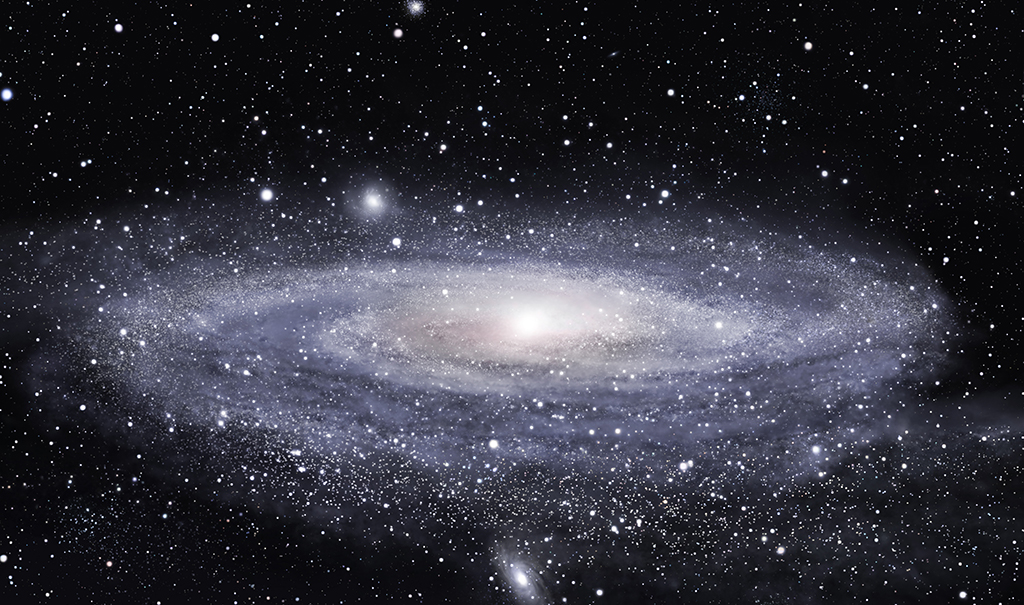
\includegraphics[width=9cm]{./img/milkyway.jpg}\end{center}
The Milky Way began as one or several small overdensities in the mass distribution in the Universe shortly after the Big Bang. Some of these overdensities were the seeds of globular clusters in which the oldest remaining stars in what is now the Milky Way formed. Nearly half the matter in the Milky Way may have come from other distant galaxies. Nonetheless, these stars and clusters now comprise the stellar halo of the Milky Way. Within a few billion years of the birth of the first stars, the mass of the Milky Way was large enough so that it was spinning relatively quickly. Due to conservation of angular momentum, this led the gaseous interstellar medium to collapse from a roughly spheroidal shape to a disk. Therefore, later generations of stars formed in this spiral disk. Most younger stars, including the Sun, are observed to be in the disk\\

Since the first stars began to form, the Milky Way has grown through both galaxy mergers (particularly early in the Milky Way's growth) and accretion of gas directly from the Galactic halo. The Milky Way is currently accreting material from several small galaxies, including two of its largest satellite galaxies, the Large and Small Magellanic Clouds, through the Magellanic Stream. Direct accretion of gas is observed in high-velocity clouds like the Smith Cloud. However, properties of the Milky Way such as stellar mass, angular momentum, and metallicity in its outermost regions suggest it has undergone no mergers with large galaxies in the last 10 billion years. This lack of recent major mergers is unusual among similar spiral galaxies; its neighbor the Andromeda Galaxy appears to have a more typical history shaped by more recent mergers with relatively large galaxies.\\

According to recent studies, the Milky Way as well as the Andromeda Galaxy lie in what in the galaxy color–magnitude diagram is known as the "green valley", a region populated by galaxies in transition from the "blue cloud" (galaxies actively forming new stars) to the "red sequence" (galaxies that lack star formation). Star-formation activity in green valley galaxies is slowing as they run out of star-forming gas in the interstellar medium. In simulated galaxies with similar properties, star formation will typically have been extinguished within about five billion years from now, even accounting for the expected, short-term increase in the rate of star formation due to the collision between both the Milky Way and the Andromeda Galaxy. In fact, measurements of other galaxies similar to the Milky Way suggest it is among the reddest and brightest spiral galaxies that are still forming new stars and it is just slightly bluer than the bluest red sequence galaxies.

\chapter{4.54 Billion years ago}
\section{Formation of planet Earth}
\vspace{2mm}\begin{center}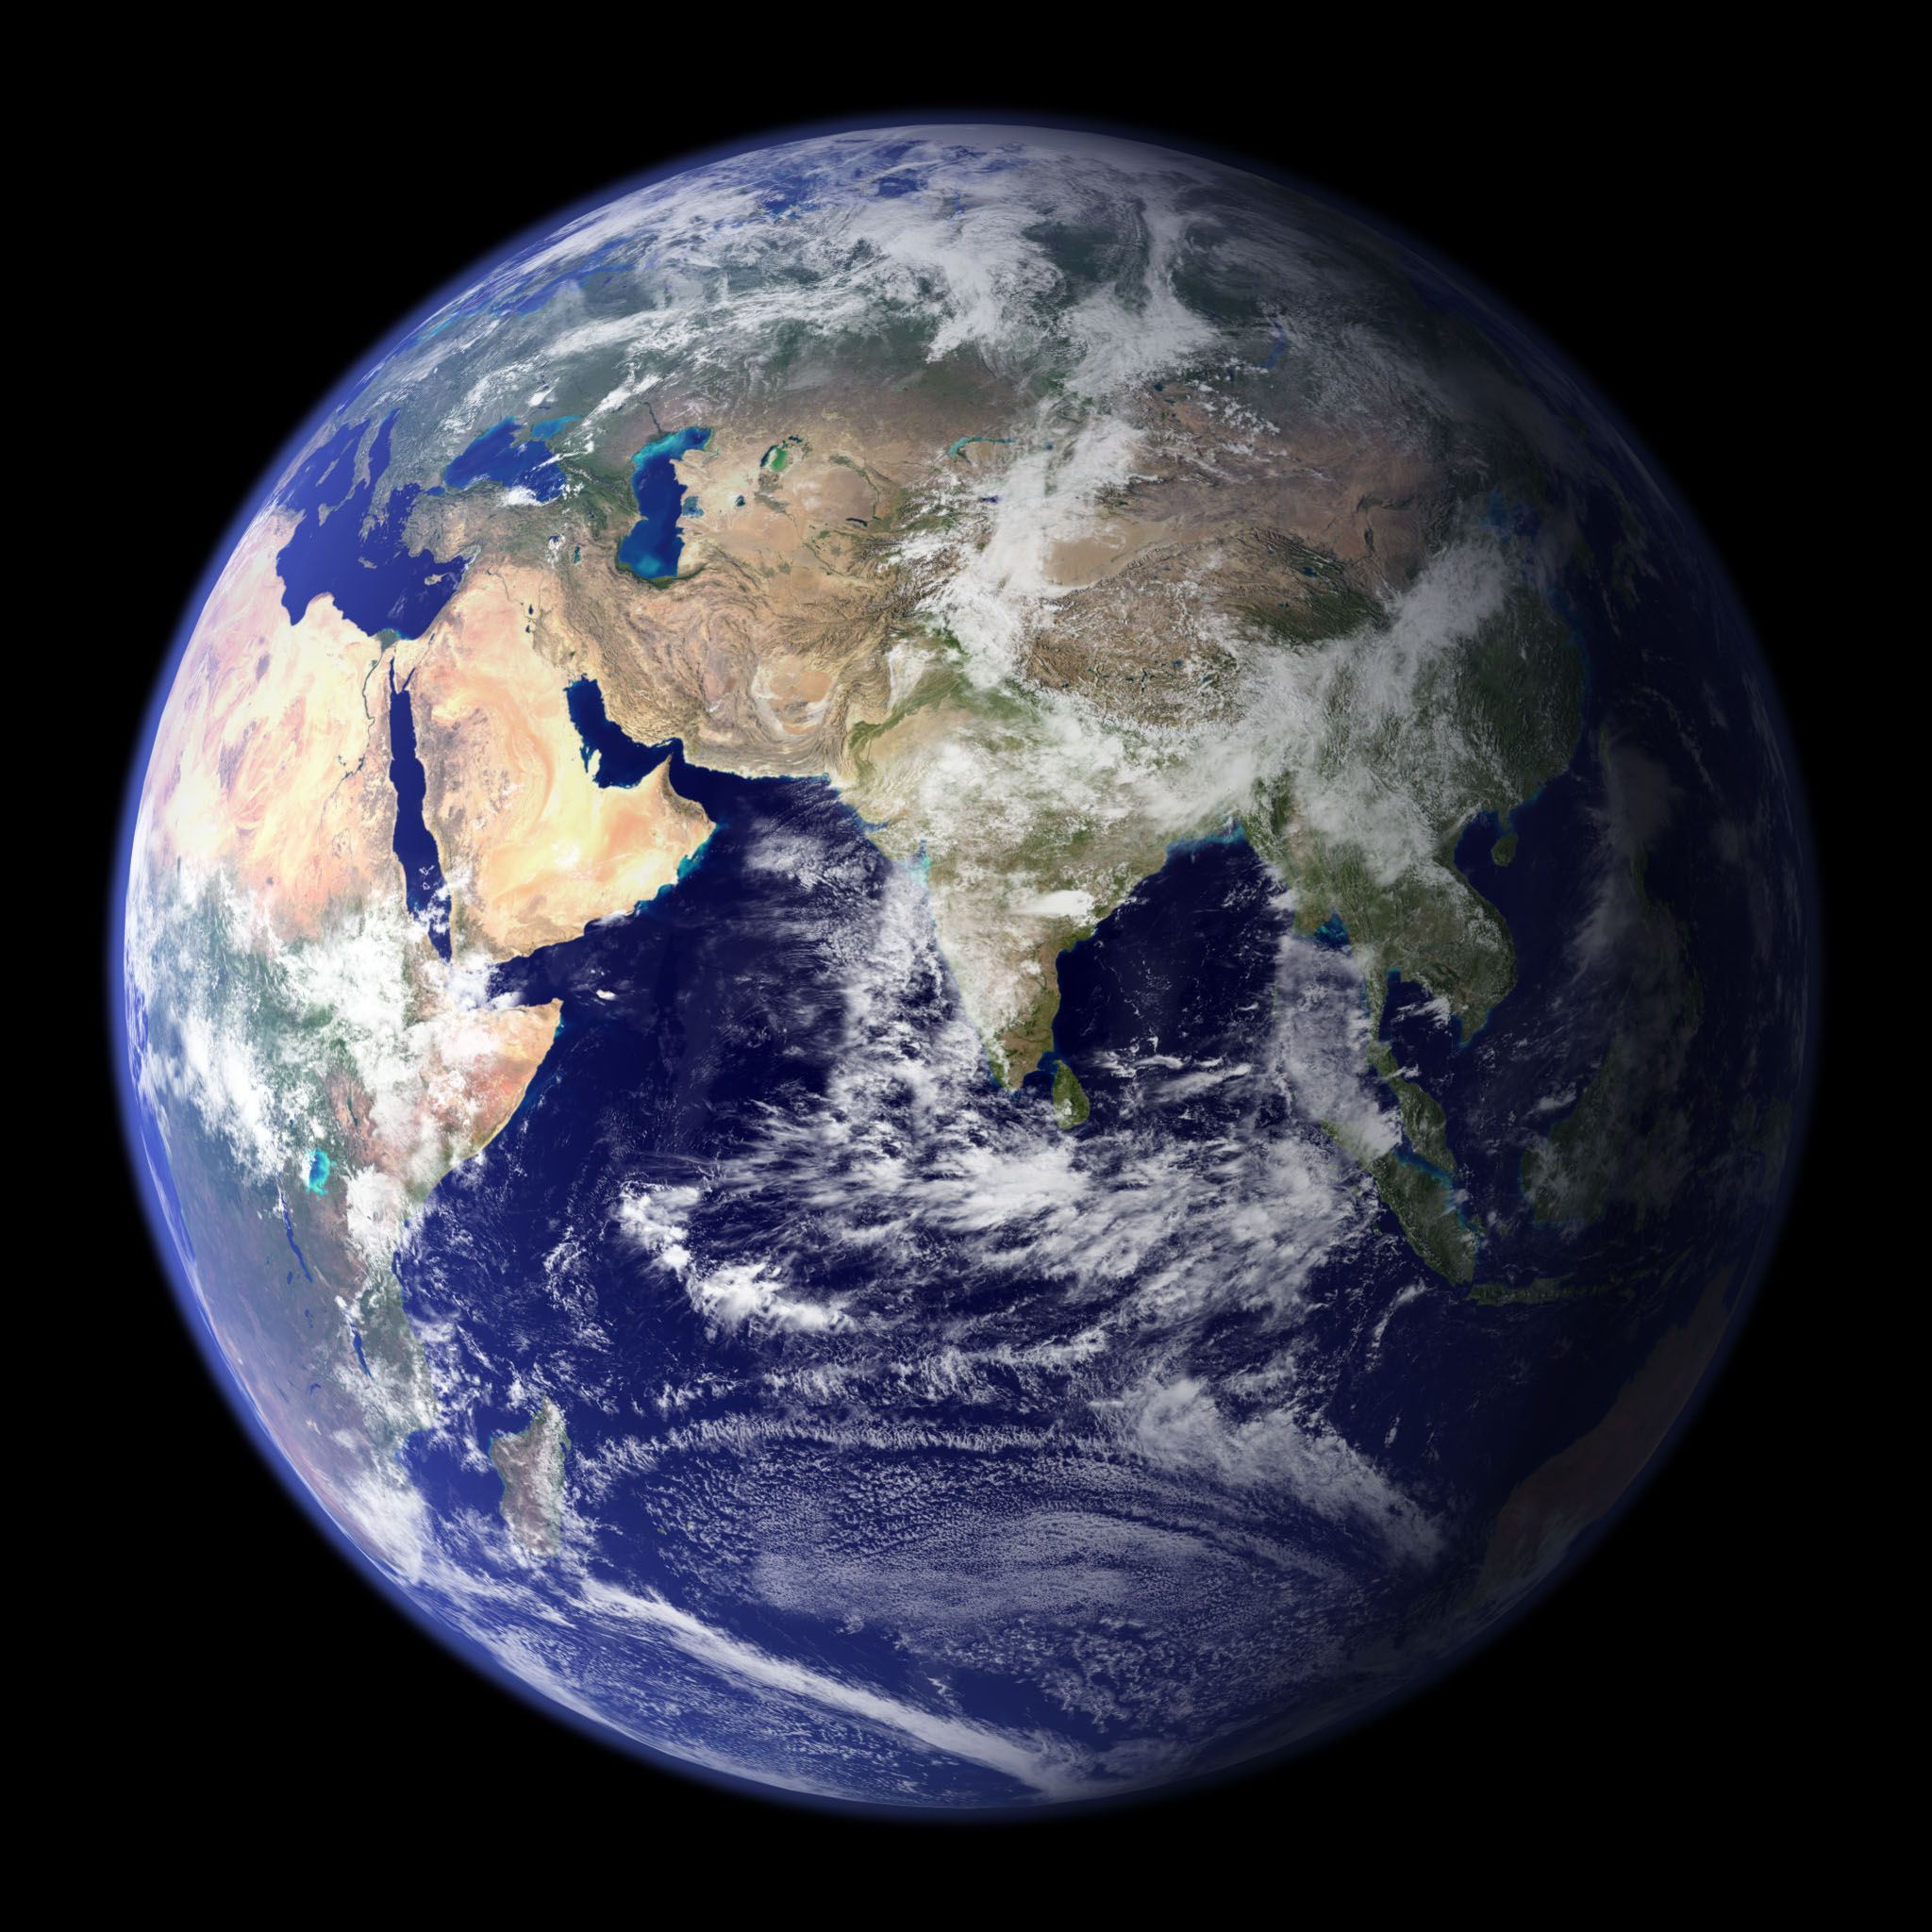
\includegraphics[width=6cm]{./img/earth.jpg}\end{center}
The history of Earth concerns the development of planet Earth from its formation to the present day. Nearly all branches of natural science have contributed to understanding of the main events of Earth's past, characterized by constant geological change and biological evolution.

The geological time scale (GTS), as defined by international convention, depicts the large spans of time from the beginning of the Earth to the present, and its divisions chronicle some definitive events of Earth history. (In the graphic: Ga means "billion years ago"; Ma, "million years ago".) Earth formed around 4.54 billion years ago, approximately one-third the age of the universe, by accretion from the solar nebula. Volcanic outgassing probably created the primordial atmosphere and then the ocean, but the early atmosphere contained almost no oxygen. Much of the Earth was molten because of frequent collisions with other bodies which led to extreme volcanism. While Earth was in its earliest stage (Early Earth), a giant impact collision with a planet-sized body named Theia is thought to have formed the Moon. Over time, the Earth cooled, causing the formation of a solid crust, and allowing liquid water on the surface.

\chapter{4.5 Billion years ago}
\section{Formation of The Moon}
\vspace{2mm}\begin{center}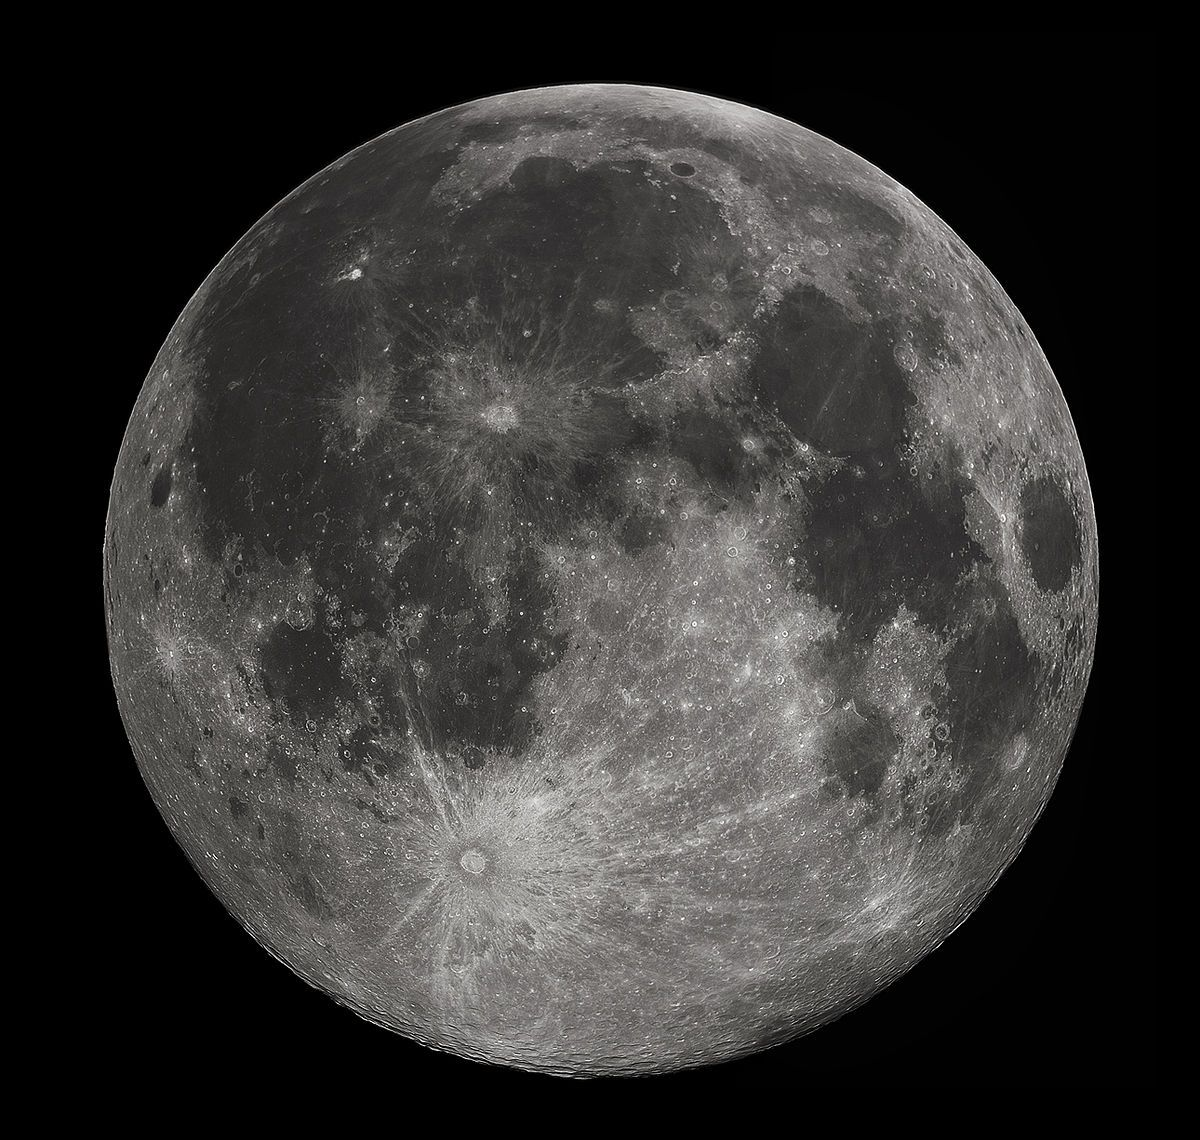
\includegraphics[width=8cm]{./img/moon.jpg}\end{center}
\textbf{Giant-impact hypothesis}:\\
The giant-impact hypothesis, sometimes called the Big Splash, or the Theia Impact suggests that the Moon formed out of the debris left over from a collision between Earth and an astronomical body the size of Mars, approximately 4.5 billion years ago, in the Hadean eon; about 20 to 100 million years after the solar system coalesced. The colliding body is sometimes called Theia, from the name of the mythical Greek Titan who was the mother of Selene, the goddess of the Moon. Analysis of lunar rocks, published in a 2016 report, suggests that the impact may have been a direct hit, causing a thorough mixing of both parent bodies.

\begin{comment}
\chapter{3.9 Billion years ago}
\section{Birth of organic life}
\vspace{2mm}\begin{center}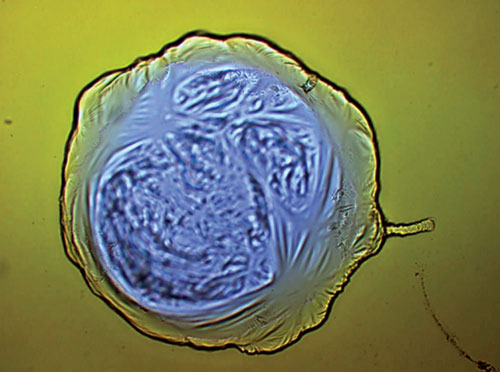
\includegraphics[width=10cm]{./img/organiclife.jpg}\end{center}
\end{comment}

\chapter{2.9 Billion years ago}
\section{Pangola Ice Age}
\vspace{2mm}\begin{center}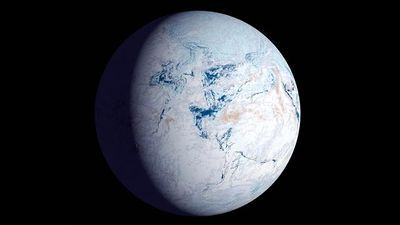
\includegraphics[width=10cm]{./img/iceage.jpg}\end{center}
The Mesoarchean is a geologic era within the Archean Eon, spanning 3,200 to 2,800 million years ago. The era is defined chronometrically and is not referenced to a specific level in a rock section on Earth. Fossils from Australia show that stromatolites have lived on Earth since the Mesoarchean. The Pongola glaciation occurred around 2,900 million years ago. The first supercontinent Vaalbara broke up during this era about 2,800 million years ago.

\chapter{1.6 Billion years ago}
\section{Eukaryotic cells appeared}
\vspace{2mm}\begin{center}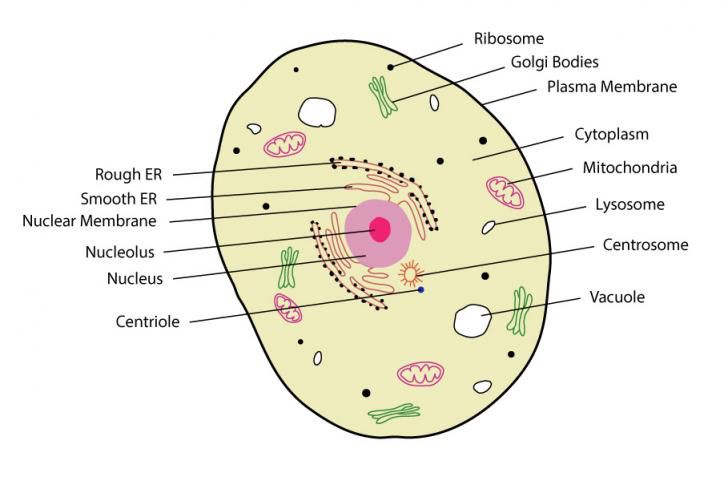
\includegraphics[width=10cm]{./img/eukaryoticCell.jpg}\end{center}
Eukaryotes are organisms whose cells have a nucleus enclosed within membranes, unlike prokaryotes (Bacteria and Archaea). Eukaryotic cells also contain other membrane-bound organelles such as mitochondria and the Golgi apparatus, and in addition, some cells of plants and algae contain chloroplasts. Unlike unicellular archaea and bacteria, eukaryotes may also be multicellular and include organisms consisting of many cell types forming different kinds of tissue. Animals and plants are the most familiar eukaryotes.

Eukaryotes can reproduce both asexually through mitosis and sexually through meiosis and gamete fusion. In mitosis, one cell divides to produce two genetically identical cells. In meiosis, DNA replication is followed by two rounds of cell division to produce four haploid daughter cells. These act as sex cells (gametes). Each gamete has just one set of chromosomes, each a unique mix of the corresponding pair of parental chromosomes resulting from genetic recombination during meiosis.

The domain Eukaryota appears to be monophyletic, and makes up one of the domains of life in the three-domain system. The two other domains, Bacteria and Archaea, are prokaryotes and have none of the above features. Eukaryotes represent a tiny minority of all living things.[8] However, due to their generally much larger size, their collective worldwide biomass is estimated to be about equal to that of prokaryotes. Eukaryotes evolved approximately 1.6–2.1 billion years ago, during the Proterozoic eon.

\part{400-300 BC}
\chapter{356 BC}
\section{July 20/21}
\subsection{Birth of Alexander III of Macedon}
\vspace{2mm}\begin{center}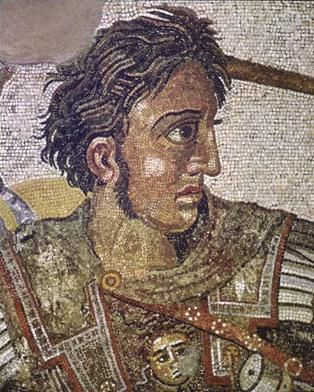
\includegraphics[width=3cm]{./img/alexanderTG.jpg}\end{center}
Alexander was born on the sixth day of the ancient Greek month of Hekatombaion, which probably corresponds to 20 July 356 BC, although the exact date is disputed, in Pella, the capital of the Kingdom of Macedon. He was the son of the king of Macedon, Philip II, and his fourth wife, Olympias, the daughter of Neoptolemus I, king of Epirus. Although Philip had seven or eight wives, Olympias was his principal wife for some time, likely because she gave birth to Alexander.


Statue of Alexander the Great in Thessaloniki, Macedonia, Greece
Several legends surround Alexander's birth and childhood. According to the ancient Greek biographer Plutarch, on the eve of the consummation of her marriage to Philip, Olympias dreamed that her womb was struck by a thunder bolt that caused a flame to spread "far and wide" before dying away. Sometime after the wedding, Philip is said to have seen himself, in a dream, securing his wife's womb with a seal engraved with a lion's image. Plutarch offered a variety of interpretations of these dreams: that Olympias was pregnant before her marriage, indicated by the sealing of her womb; or that Alexander's father was Zeus. Ancient commentators were divided about whether the ambitious Olympias promulgated the story of Alexander's divine parentage, variously claiming that she had told Alexander, or that she dismissed the suggestion as impious


										%6th century
										
	
\part{6th century}
\chapter{570}
\section{}
\subsection{Birth of Muhammad}
\vspace{2mm}\begin{center}
\includegraphics[width=7cm]{./img/muhammad.jpg}\end{center}
Abu al-Qasim Muhammad ibn'Abd Allah ibn 'Abd al-Muttalib ibn Hashim, was born about the year 570 and his birthday is believed to be in the month of Rabi' al-awwal. He belonged to the Banu Hashim clan, part of the Quraysh tribe, and was one of Mecca's prominent families, although it appears less prosperous during Muhammad's early lifetime. Tradition places the year of Muhammad's birth as corresponding with the Year of the Elephant, which is named after the failed destruction of Mecca that year by the Abraha, Yemen's king, who supplemented his army with elephants. Alternatively some 20th century scholars have suggested different years, such as 568 or 569.

\chapter{}
\section{}
\subsection{First Bubonic Plague pandemic}
\vspace{2mm}\begin{center}
\includegraphics[width=5cm]{./img/skull.png}\end{center}
The first recorded epidemic affected the Eastern Roman Empire (Byzantine Empire) and was named the Plague of Justinian after emperor Justinian I, who was infected but survived through extensive treatment. The pandemic resulted in the deaths of an estimated 25 million (6th century outbreak) to 50 million people (two centuries of recurrence). The historian Procopius wrote, in Volume II of History of the Wars, of his personal encounter with the plague and the effect it had on the rising empire. In the spring of 542, the plague arrived in Constantinople, working its way from port city to port city and spreading around the Mediterranean Sea, later migrating inland eastward into Asia Minor and west into Greece and Italy. Because the infectious disease spread inland by the transferring of merchandise through Justinian’s efforts in acquiring luxurious goods of the time and exporting supplies, his capital became the leading exporter of the bubonic plague. Procopius, in his work Secret History, declared that Justinian was a demon of an emperor who either created the plague himself or was being punished for his sinfulness


										%12th century
										
	
\part{12th century}
\chapter{1162}
\section{}
\subsection{Birth of Genghis Khan}
\vspace{2mm}\begin{center}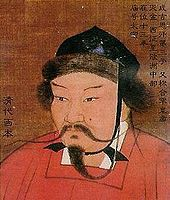
\includegraphics[width=5cm]{./img/gengishKhan.jpg}\end{center}
Little is known about Genghis Khan's early life, due to the lack of contemporary written records. The few sources that give insight into this period often contradict.

Genghis Khan's birth name, Temüjin, was derived from the Mongol word temür meaning "of iron", while jin denotes agency. Temüjin thus means "blacksmith".

Genghis Khan was probably born in 1162 in Delüün Boldog, near the mountain Burkhan Khaldun and the rivers Onon and Kherlen in modern-day northern Mongolia, close to the current capital Ulaanbaatar. The Secret History of the Mongols reports that Temüjin was born grasping a blood clot in his fist, a traditional sign that he was destined to become a great leader. He was the second son of his father Yesügei who was a Kiyad chief prominent in the Khamag Mongol confederation and an ally of Toghrul of the Keraite tribe. Temüjin was the first son of his mother Hoelun. According to the Secret History, Temüjin was named after the Tatar chief Temüjin-üge whom his father had just captured.


										%13th century
										
	
\part{13th century}
\section{}
\subsection{Renaissance}
\vspace{2mm}\begin{center}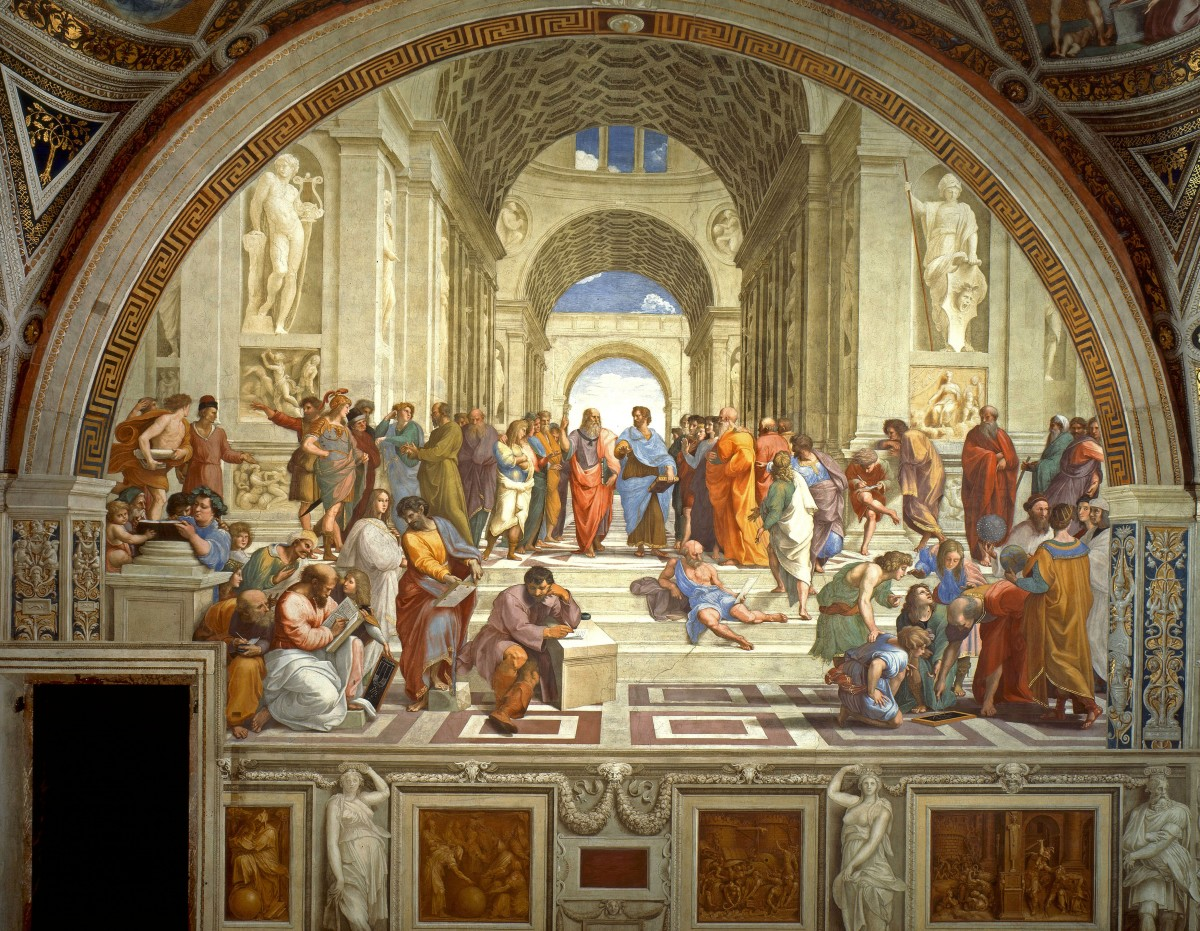
\includegraphics[width=8cm]{./img/renaissance.jpg}\end{center}
Many argue that the ideas characterizing the Renaissance had their origin in late 13th-century Florence, in particular with the writings of Dante Alighieri (1265–1321) and Petrarch (1304–1374), as well as the paintings of Giotto di Bondone (1267–1337). Some writers date the Renaissance quite precisely; one proposed starting point is 1401, when the rival geniuses Lorenzo Ghiberti and Filippo Brunelleschi competed for the contract to build the bronze doors for the Baptistery of the Florence Cathedral (Ghiberti won). Others see more general competition between artists and polymaths such as Brunelleschi, Ghiberti, Donatello, and Masaccio for artistic commissions as sparking the creativity of the Renaissance. Yet it remains much debated why the Renaissance began in Italy, and why it began when it did. Accordingly, several theories have been put forward to explain its origins.

During the Renaissance, money and art went hand in hand. Artists depended entirely on patrons while the patrons needed money to foster artistic talent. Wealth was brought to Italy in the 14th, 15th, and 16th centuries by expanding trade into Asia and Europe. Silver mining in Tyrol increased the flow of money. Luxuries from the Eastern world, brought home during the Crusades, increased the prosperity of Genoa and Venice.

Jules Michelet defined the 16th-century Renaissance in France as a period in Europe's cultural history that represented a break from the Middle Ages, creating a modern understanding of humanity and its place in the world


\part{14th century}
\chapter{1300}
\section{}
\subsection{Second Bubonic Plague pandemic}
\vspace{2mm}\begin{center}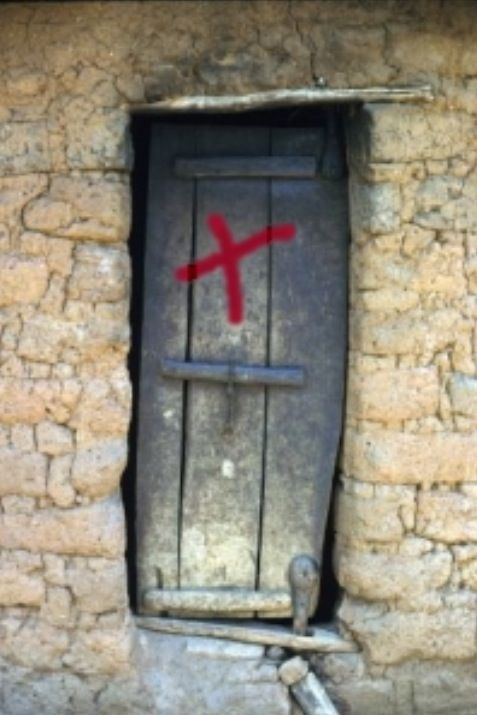
\includegraphics[width=2cm]{./img/bubonicDoor.jpg}\end{center}
In the Late Middle Ages (1340–1400) Europe experienced the most deadly disease outbreak in history when the Black Death, the infamous pandemic of bubonic plague, hit in 1347, killing a third of the European human population. Some historians believe that society subsequently became more violent as the mass mortality rate cheapened life and thus increased warfare, crime, popular revolt, waves of flagellants, and persecution. The Black Death originated in Central Asia and spread from Italy and then throughout other European countries. Arab historians Ibn Al-Wardni and Almaqrizi believed the Black Death originated in Mongolia. Chinese records also showed a huge outbreak in Mongolia in the early 1330s. Research published in 2002 suggests that it began in early 1346 in the steppe region, where a plague reservoir stretches from the northwestern shore of the Caspian Sea into southern Russia. The Mongols had cut off the trade route, the Silk Road, between China and Europe which halted the spread of the Black Death from eastern Russia to Western Europe. The epidemic began with an attack that Mongols launched on the Italian merchants' last trading station in the region, Caffa in the Crimea. In late 1346, plague broke out among the besiegers and from them penetrated into the town. When spring arrived, the Italian merchants fled on their ships, unknowingly carrying the Black Death. Carried by the fleas on rats, the plague initially spread to humans near the Black Sea and then outwards to the rest of Europe as a result of people fleeing from one area to another.


										%15th century
										
	
\part{15th century}

\chapter{1453}
\section{May 29}
\subsection{The Fall of Constantinople}
\vspace{2mm}\begin{center}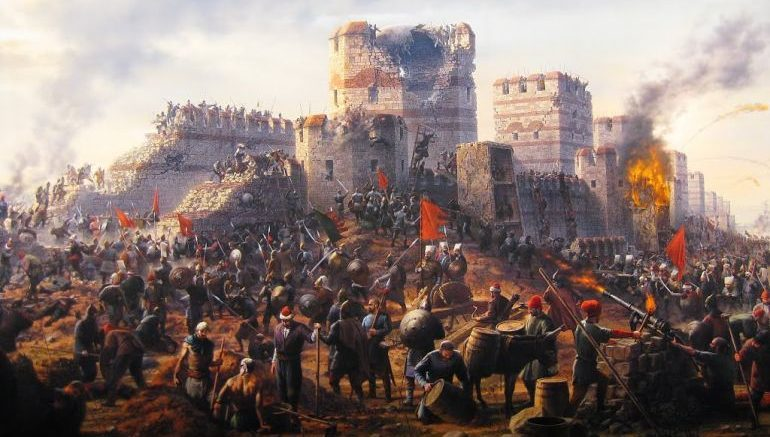
\includegraphics[width=4cm]{./img/fallofConstantpl.jpg}\end{center}
The Fall of Constantinople was the capture of the capital of the Byzantine Empire by an invading Ottoman army on 29 May 1453. The attackers were commanded by the 21-year-old Sultan Mehmed II, who defeated an army commanded by Emperor Constantine XI Palaiologos and took control of the imperial capital, ending a 53-day siege that began on 6 April 1453. After conquering the city, Sultan Mehmed transferred the capital of his Empire from Edirne to Constantinople and established his court there.

The capture of the city (and two other Byzantine splinter territories soon thereafter) marked the end of the Byzantine Empire, a continuation of the Roman Empire, an imperial state dating to 27 BC, which had lasted for nearly 1,500 years. The conquest of Constantinople also dealt a massive blow to Christendom, as the Muslim Ottoman armies thereafter were left unchecked to advance into Europe without an adversary to their rear.

It was also a watershed moment in military history. Since ancient times, cities had used ramparts and city walls to protect themselves from invaders, and Constantinople's substantial fortifications had been a model followed by cities throughout the Mediterranean region and Europe. The Ottomans ultimately prevailed due to the use of gunpowder (which powered formidable cannons).

The conquest of the city of Constantinople and the end of the Byzantine Empire was a key event in the Late Middle Ages which also marks, for some historians, the end of the Medieval period.

\chapter{1468}
\section{February 2}
\subsection{Birth of Johannes Gutenberg}
\vspace{2mm}\begin{center}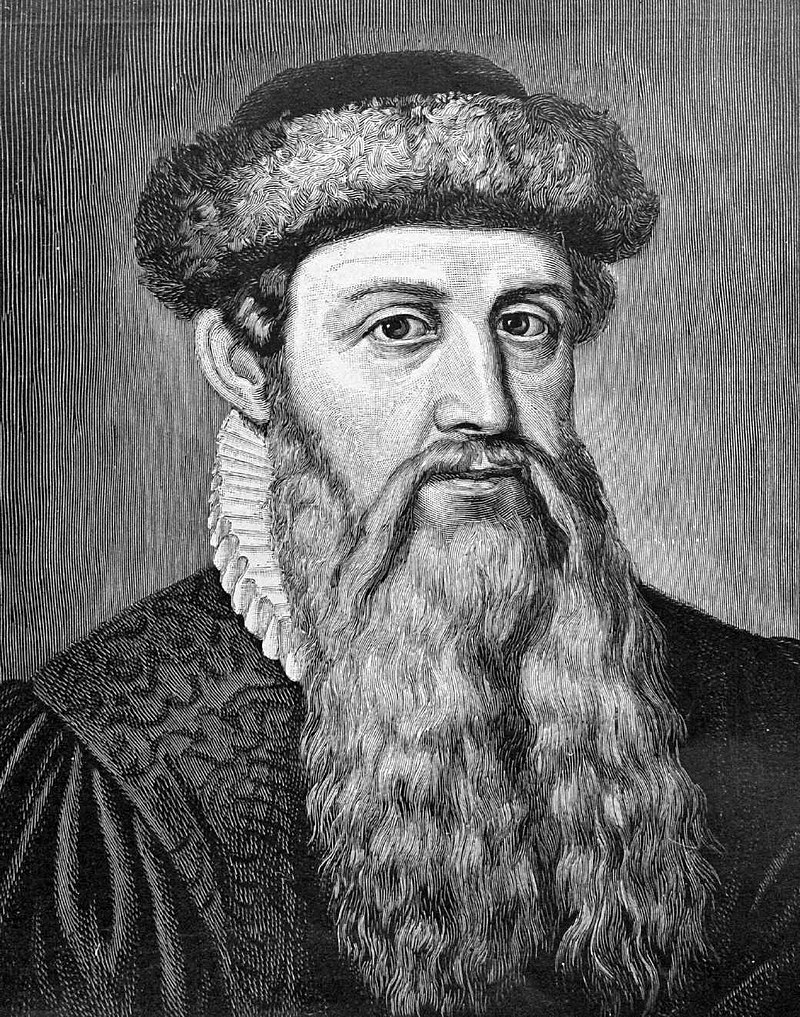
\includegraphics[width=5cm]{./img/gutenberg.jpg}\end{center}
Johannes Gensfleisch zur Laden zum Gutenberg (February 3, 1468) was a German blacksmith, goldsmith, inventor, printer, and publisher who introduced printing to Europe with the printing press. His introduction of mechanical movable type printing to Europe started the Printing Revolution and is regarded as a milestone of the second millennium, ushering in the modern period of human history. It played a key role in the development of the Renaissance, Reformation, the Age of Enlightenment, and the scientific revolution and laid the material basis for the modern knowledge-based economy and the spread of learning to the masses.

\chapter{1492}
\section{December 26}
\subsection{First Spanish settlement La Navidad in the New World}
\vspace{2mm}\begin{center}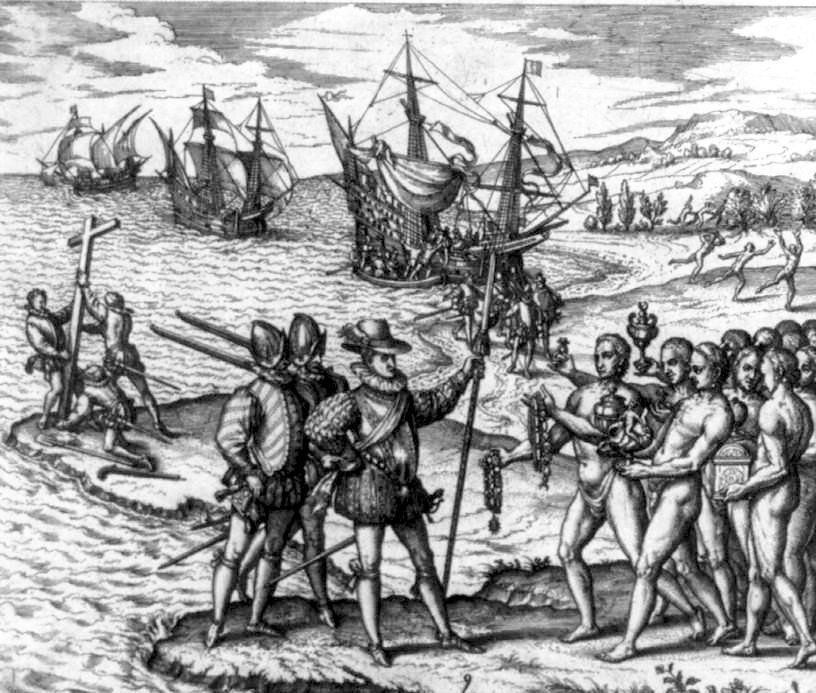
\includegraphics[width=10cm]{./img/lanavidad.jpg}\end{center}
La Navidad was a settlement that Christopher Columbus and his men established in present-day Haiti in 1492 from the remains of the Spanish ship, the Santa María. La Navidad was the first European colony established in the New World during the Age of Discovery, though it was destroyed the following year.




										%16th century
										
										
\part{16th century}
\chapter{1543}
\section{}
\subsection{Modern scientific revolution}
\vspace{2mm}\begin{center}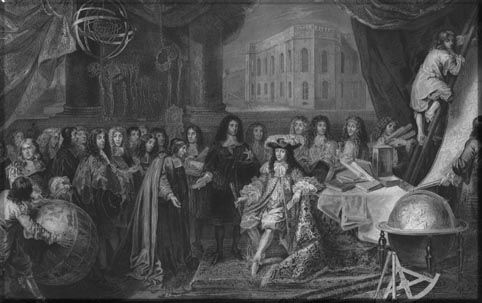
\includegraphics[width=10cm]{./img/screvolution.jpg}\end{center}
The Scientific Revolution was a series of events that marked the emergence of modern science during the early modern period, when developments in mathematics, physics, astronomy, biology (including human anatomy) and chemistry transformed the views of society about nature. The Scientific Revolution took place in Europe towards the end of the Renaissance period and continued through the late 18th century, influencing the intellectual social movement known as the Enlightenment. While its dates are debated, the publication in 1543 of Nicolaus Copernicus's De revolutionibus orbium coelestium (On the Revolutions of the Heavenly Spheres) is often cited as marking the beginning of the Scientific Revolution.


										%17th century
		
\part{17th century}
\chapter{1643}
\section{January 04}
\subsection{Birth of Sir Isaac Newton}
\vspace{2mm}\begin{center}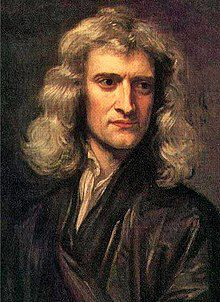
\includegraphics[width=5cm]{./img/isaacNewton.jpg}\end{center}
Sir Isaac Newton was an English mathematician, physicist, astronomer, theologian, and author (described in his own day as a "natural philosopher") who is widely recognized as one of the most influential scientists of all time, and a key figure in the scientific revolution. His book Philosophiæ Naturalis Principia Mathematica ("Mathematical Principles of Natural Philosophy"), first published in 1687, laid the foundations of classical mechanics. Newton also made seminal contributions to optics, and shares credit with Gottfried Wilhelm Leibniz for developing the infinitesimal calculus.


										%18th century
										
\part{18th century}
\chapter{1760}
\section{}
\subsection{Industrial revolution}
\vspace{2mm}\begin{center}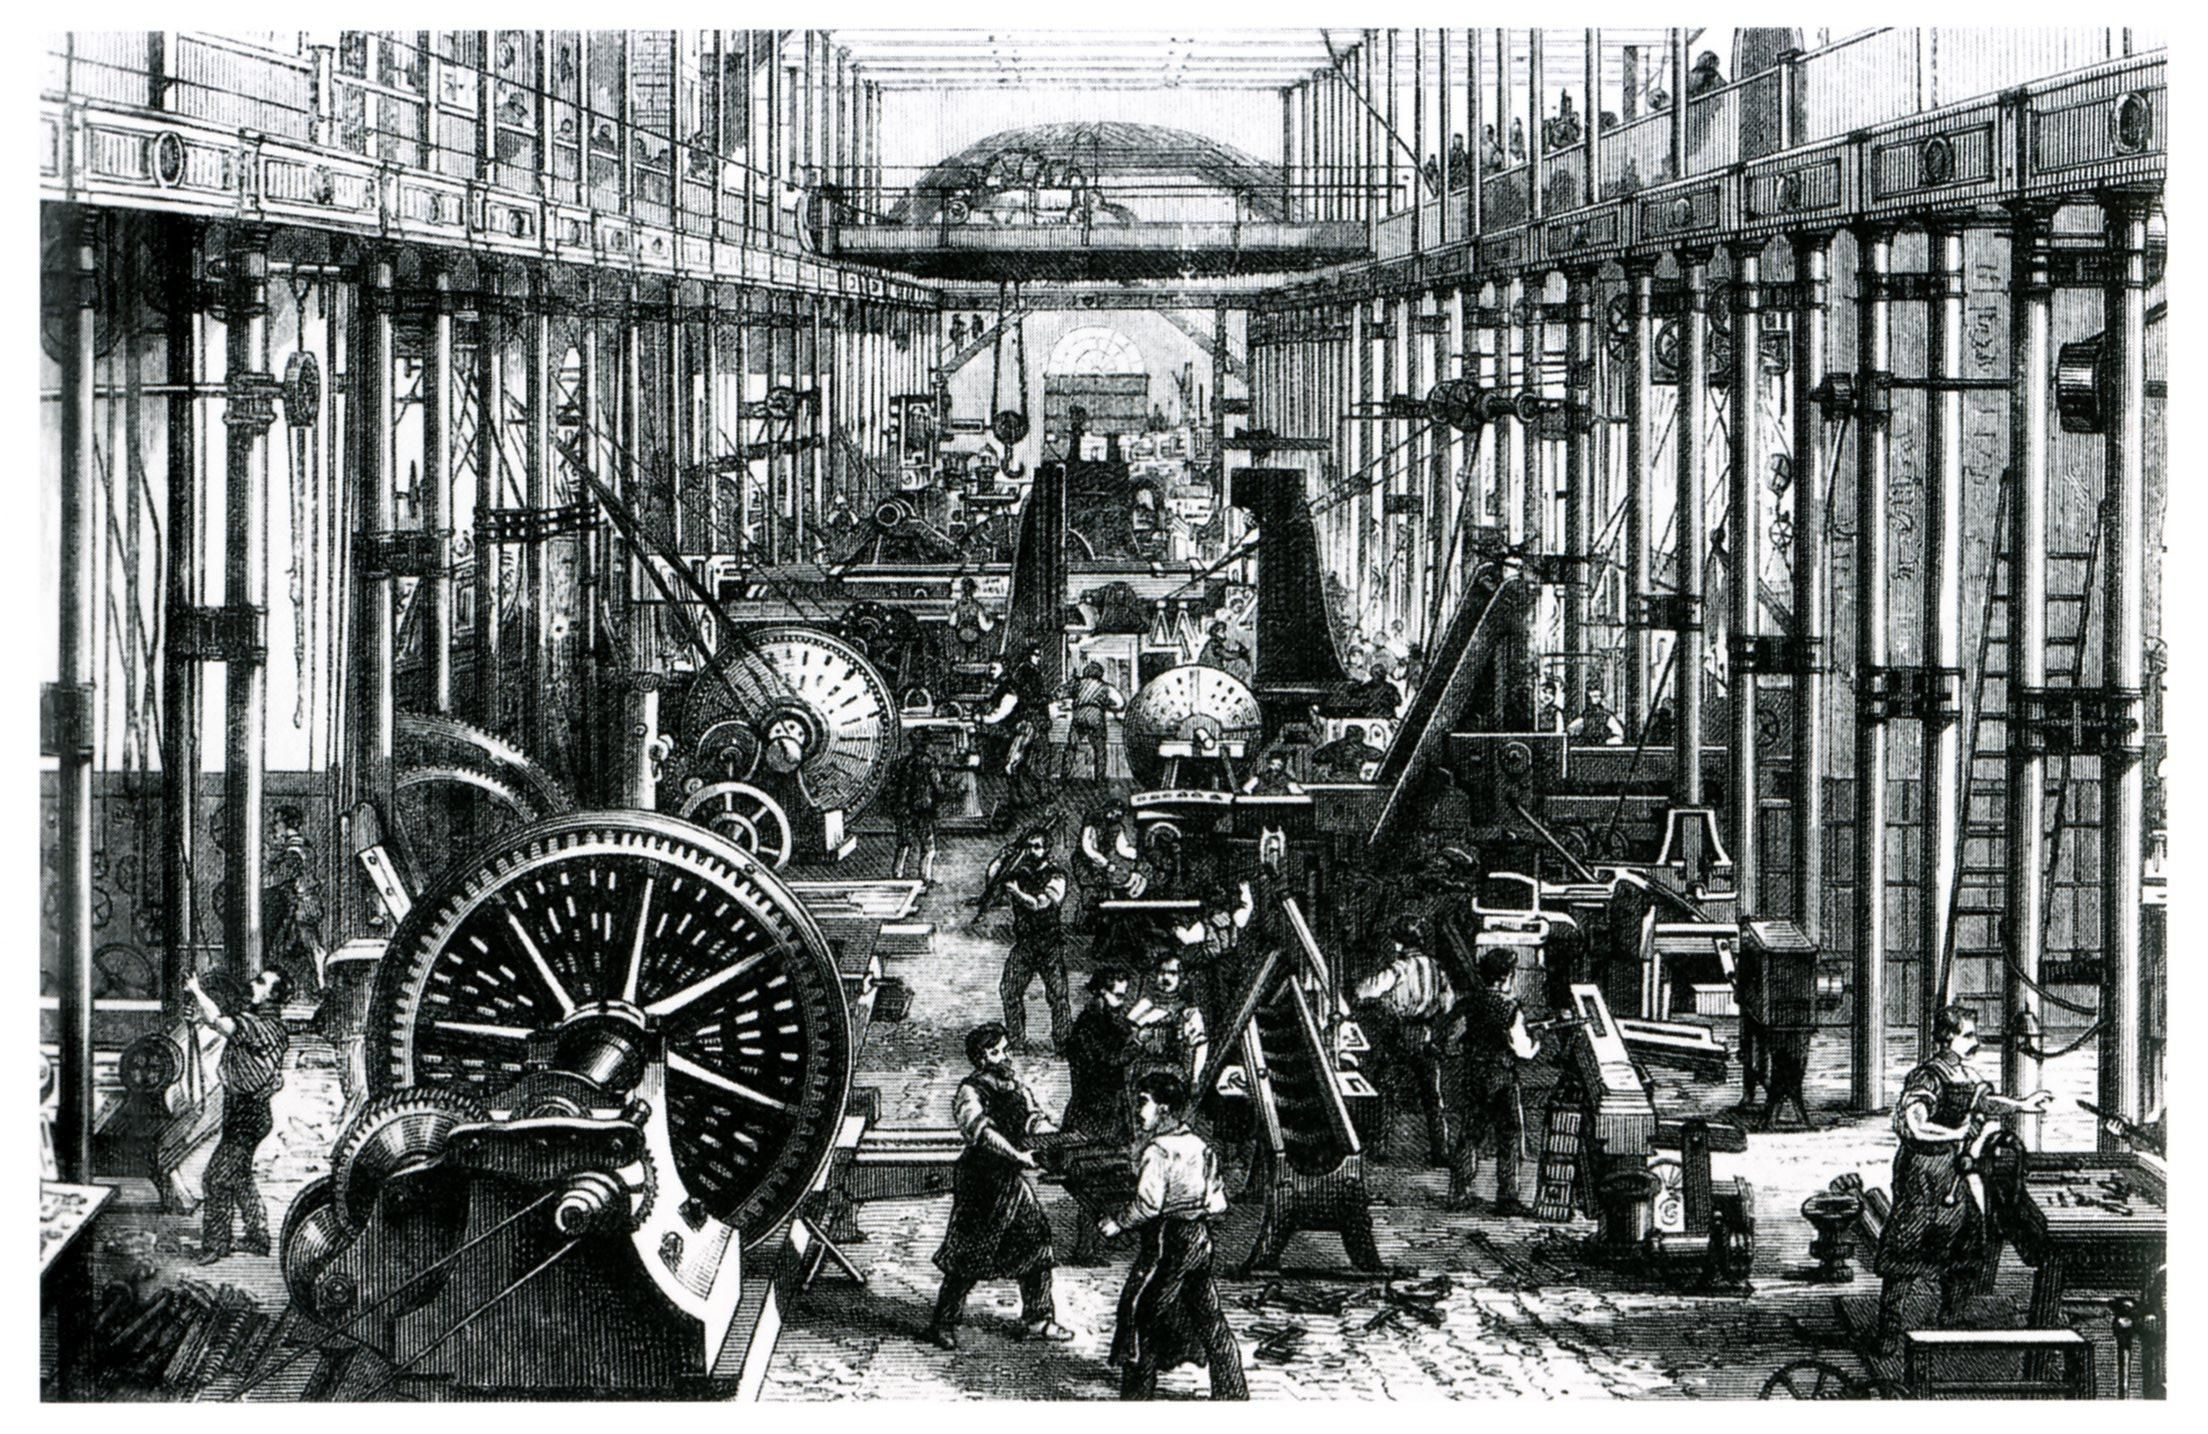
\includegraphics[width=10cm]{./img/industrevolution.jpg}\end{center}
The Industrial Revolution was the transition to new manufacturing processes in Europe and the US, in the period from about 1760 to sometime between 1820 and 1840. This transition included going from hand production methods to machines, new chemical manufacturing and iron production processes, the increasing use of steam power, the development of machine tools and the rise of the factory system. The Industrial Revolution also led to an unprecedented rise in the rate of population growth.

\chapter{1766}
\section{December 25}
\subsection{George Washington's crossing of the Delaware River}
\vspace{2mm}\begin{center}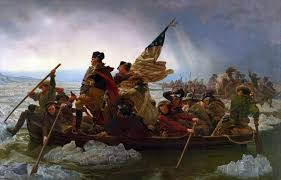
\includegraphics[width=10cm]{./img/crossingDelaware.jpg}\end{center}
George Washington's crossing of the Delaware River, which occurred on the night of December 25–26, 1776, during the American Revolutionary War, was the first move in a surprise attack organized by George Washington against the Hessian forces in Trenton, New Jersey, on the morning of December 26. Planned in partial secrecy, Washington led a column of Continental Army troops across the icy Delaware River in a logistically challenging and dangerous operation. Other planned crossings in support of the operation were either called off or ineffective, but this did not prevent Washington from surprising and defeating the troops of Johann Rall quartered in Trenton. The army crossed the river back to Pennsylvania, this time laden with prisoners and military stores taken as a result of the battle.


										%19th century
										
			
\part{19th century}
\chapter{1821}
\section{December 25}
\subsection{Birth of Clara Harlowe Barton}
\vspace{2mm}\begin{center}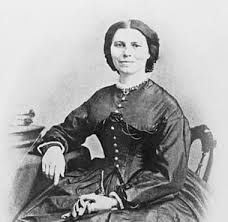
\includegraphics[width=7cm]{./img/claraBarton.jpg}\end{center}
Clarissa "Clara" Harlowe Barton (December 25, 1821 – April 12, 1912) was a pioneering nurse who founded the American Red Cross. She was a hospital nurse in the American Civil War, a teacher, and patent clerk. Nursing education was not very formalized at that time and she did not attend nursing school, so she provided self-taught nursing care. Barton is noteworthy for doing humanitarian work at a time when relatively few women worked outside the home. She was inducted into the National Women's Hall of Fame in 1973.

\chapter{Mid 19th century}
\section{}
\subsection{Third Bubonic Plague pandemic}
%\vspace{2mm}\begin{center}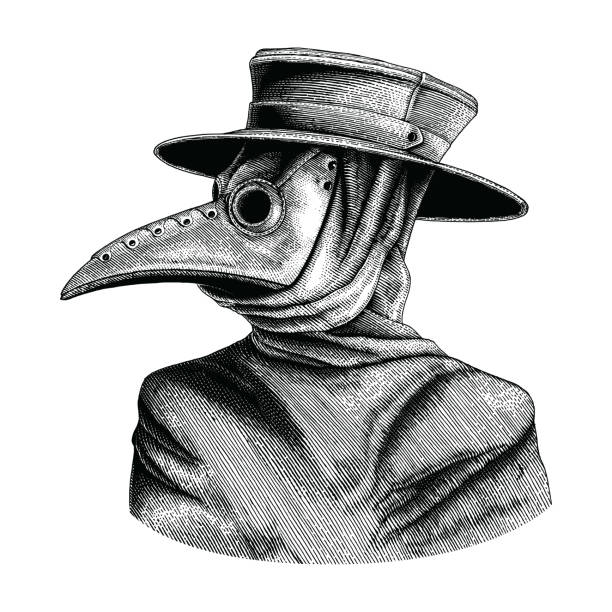
\includegraphics[width=1cm]{./img/bubonicDoc.jpg}\end{center}
The plague resurfaced for a third time in the mid-19th century. Like the two previous outbreaks, this one also originated in Eastern Asia, most likely in Yunnan Province of China, where there are several natural plague foci. The initial outbreaks occurred in the second half of the eighteenth century. The disease remained localized in Southwest China for several years before spreading. In the city of Canton, beginning in January 1894, the disease killed 80,000 people by June. Daily water-traffic with the nearby city of Hong Kong rapidly spread the plague there, killing over 2,400 within two months.

Also known as the modern pandemic, the third pandemic spread the disease to port cities throughout the world in the second half of the 19th century and early 20th century via shipping routes. The plague inflicted people in Chinatown in San Francisco from 1900-1904, and the people of Oakland and east bay again from 1907-1909. During the outbreak from 1900-1904 in San Francisco is when authorities made permanent the Chinese Exclusion Act. This law was originally signed into existence by President Chester A. Arthur in 1882. The Chinese Exclusion Act was supposed to last for ten years but was renewed in 1892 with the Geary Act and subsequently made permanent in 1902 during the outbreak of plague in Chinatown, San Francisco. The last major outbreak in the United States occurred in Los Angeles in 1924, though the disease is still present in wild rodents, and can be passed to humans that come in contact with them. According to the World Health Organization, the pandemic was considered active until 1959, when worldwide casualties dropped to 200 per year. In 1994, a plague outbreak in five Indian states caused an estimated 700 infections (including 52 deaths) and triggered a large migration of Indians within India as they tried to avoid the plague.

\chapter{1896}
\section{April 6-15}
\subsection{1896 Summer Olympics}
\vspace{2mm}\begin{center}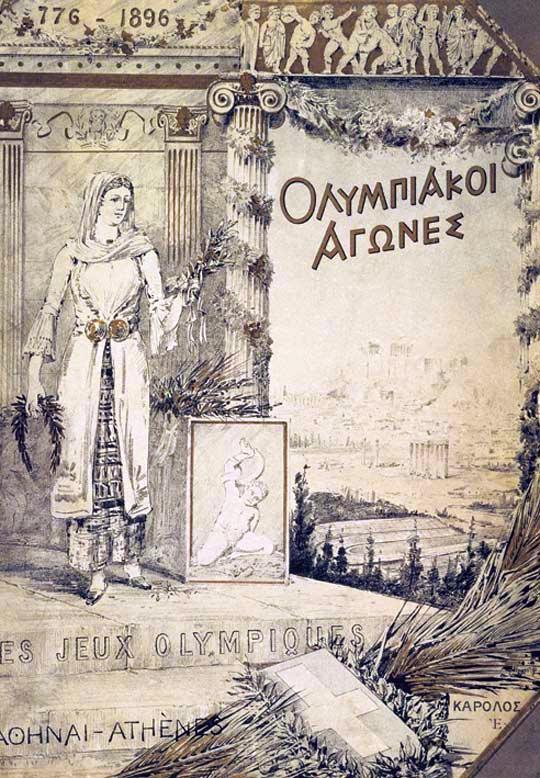
\includegraphics[width=5cm]{./img/olgames.jpg}\end{center}
The 1896 Summer Olympics officially known as the Games of the I Olympiad, was the first international Olympic Games held in modern history. Organised by the International Olympic Committee (IOC), which had been created by Pierre de Coubertin, it was held in Athens, Greece, from 6 to 15 April 1896.

Winners were given a silver medal, while runners-up received a copper medal. Retroactively, the IOC has converted these to gold and silver, and awarded bronze medals to third placed athletes. Ten of the 14 participating nations earned medals. The United States won the most gold medals, 11, host nation Greece won the most medals overall, 46. The highlight for the Greeks was the marathon victory by their compatriot Spyridon Louis. The most successful competitor was German wrestler and gymnast Carl Schuhmann, who won four events.


\chapter{1879}
\section{March 14}
\subsection{Birth of Albert Einstein}
\vspace{2mm}\begin{center}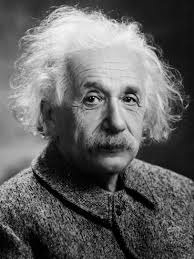
\includegraphics[width=6cm]{./img/einstein.jpg}\end{center}
Albert Einstein (14 March 1879 – 18 April 1955) was a German-born theoretical physicist who developed the theory of relativity, one of the two pillars of modern physics (alongside quantum mechanics). His work is also known for its influence on the philosophy of science. He is best known to the general public for his mass–energy equivalence formula E = mc2, which has been dubbed "the world's most famous equation". He received the 1921 Nobel Prize in Physics "for his services to theoretical physics, and especially for his discovery of the law of the photoelectric effect", a pivotal step in the development of quantum theory.

\chapter{1887}
\section{January 28}
\subsection{Construction of the Eiffel Tower begins}
\vspace{2mm}\begin{center}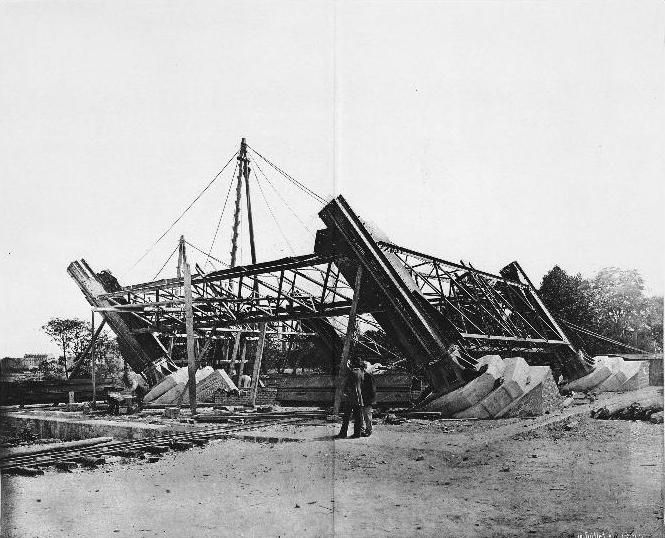
\includegraphics[width=10cm]{./img/eiffelTowerConstruction.jpg}\end{center}
Work on the foundations started on 28 January 1887. Those for the east and south legs were straightforward, with each leg resting on four 2 m (6.6 ft) concrete slabs, one for each of the principal girders of each leg. The west and north legs, being closer to the river Seine, were more complicated: each slab needed two piles installed by using compressed-air caissons 15 m (49 ft) long and 6 m (20 ft) in diameter driven to a depth of 22 m (72 ft) to support the concrete slabs, which were 6 m (20 ft) thick. Each of these slabs supported a block of limestone with an inclined top to bear a supporting shoe for the ironwork.

\chapter{1889}
\section{April 16}
\subsection{Birth of Charles Chaplin}
\vspace{2mm}\begin{center}
\includegraphics[width=7cm]{./img/charlieChaplin.jpg}\end{center}
Charles Spencer Chaplin was born on 16 April 1889 to Hannah Chaplin (born Hannah Harriet Pedlingham Hill) and Charles Chaplin Sr. There is no official record of his birth, although Chaplin believed he was born at East Street, Walworth, in South London. His mother and father had married four years previously, at which time Charles Sr. became the legal guardian of Hannah's illegitimate son, Sydney John Hill. At the time of his birth, Chaplin's parents were both music hall entertainers. Hannah, the daughter of a shoemaker, had a brief and unsuccessful career under the stage name Lily Harley, while Charles Sr., a butcher's son, was a popular singer. Although they never divorced, Chaplin's parents were estranged by around 1891. The following year, Hannah gave birth to a third son – George Wheeler Dryden – fathered by the music hall entertainer Leo Dryden. The child was taken by Dryden at six months old, and did not re-enter Chaplin's life for 30 years.

\section{September 23}
\subsection{Nintendo is founded}
\vspace{2mm}\begin{center}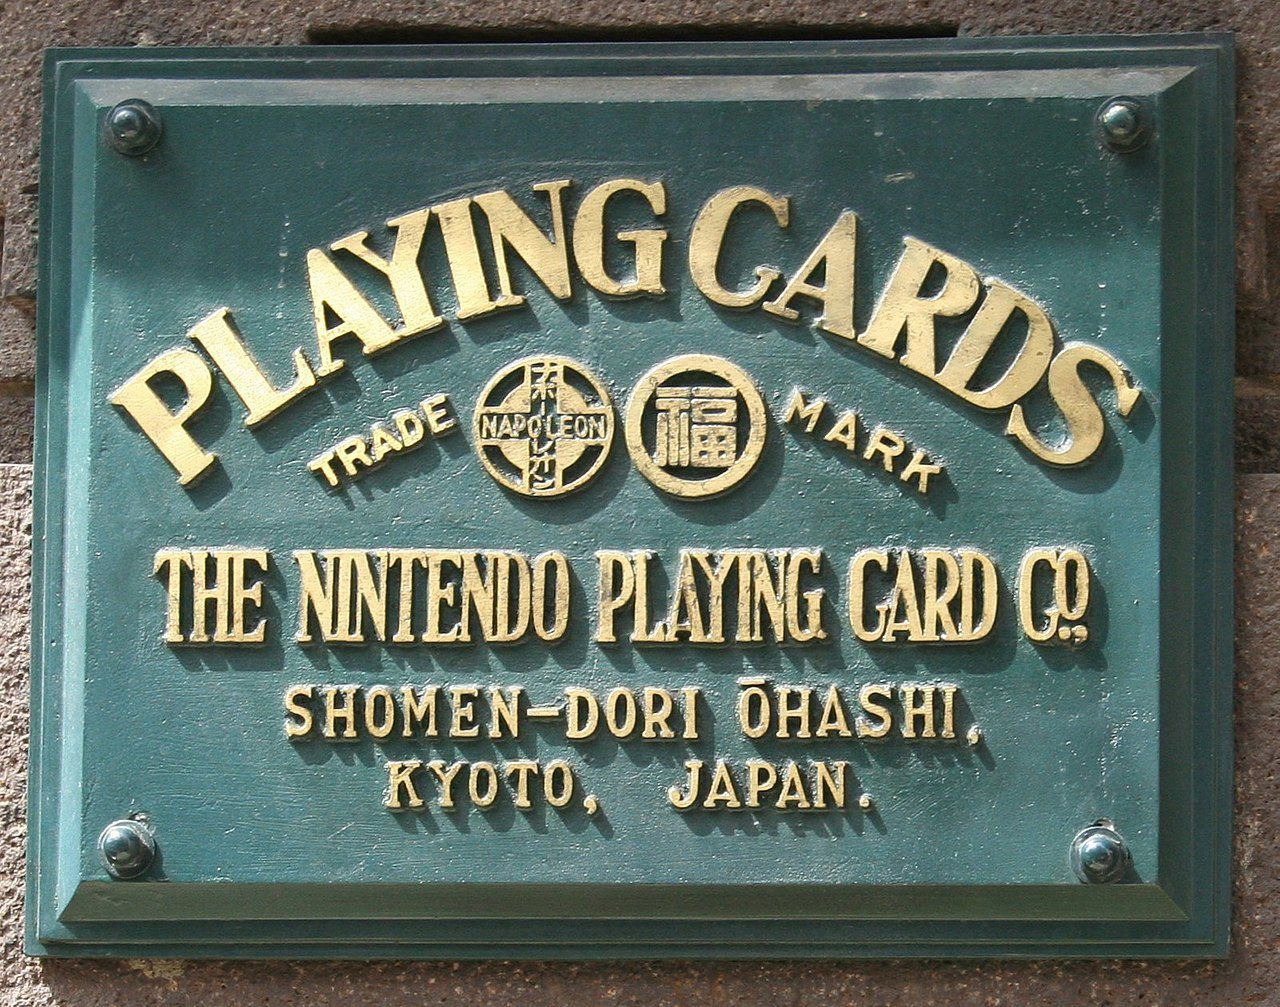
\includegraphics[width=10cm]{./img/nintendoFounded.jpg}\end{center}
Nintendo was founded as a playing card company by Fusajiro Yamauchi on 23 September 1889. Based in Kyoto, the business produced and marketed Hanafuda cards. The handmade cards soon became popular, and Yamauchi hired assistants to mass-produce cards to satisfy demand. In 1949, the company adopted the name Nintendo Karuta Co., Ltd., doing business as The Nintendo Playing Card Co. outside Japan. Nintendo continues to manufacture playing cards in Japan and organises its own contract bridge tournament called the "Nintendo Cup". The word Nintendo can be translated as "leave luck to heaven", or alternatively as "the temple of free hanafuda"

\chapter{1892}
\section{January 3}
\subsection{Birth of J.R.R Tolkien}
\vspace{2mm}\begin{center}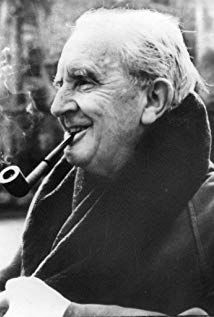
\includegraphics[width=5cm]{./img/jrrtolkien.jpg}\end{center}
John Ronald Reuel Tolkien, (3 January 1892 – 2 September 1973) was an English writer, poet, philologist, and university professor who is best known as the author of the classic high fantasy works The Hobbit, The Lord of the Rings, and The Silmarillion.

He served as the Rawlinson and Bosworth Professor of Anglo-Saxon and Fellow of Pembroke College, Oxford, from 1925 to 1945 and Merton Professor of English Language and Literature and Fellow of Merton College, Oxford, from 1945 to 1959. He was at one time a close friend of C. S. Lewis, they were both members of the informal literary discussion group known as the Inklings. Tolkien was appointed a Commander of the Order of the British Empire by Queen Elizabeth II on 28 March 1972.




										%20th century
										
			
\part{20th Century}
\chapter{Year 1903}
\section{June 16}
\subsection{Ford is founded}

\section{December 17}
\subsection{First flight by the Wright brothers}
\vspace{2mm}\begin{center}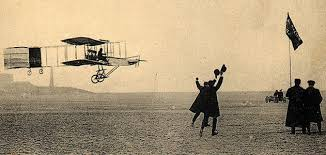
\includegraphics[width=10cm]{./img/flight.jpg}\end{center}
The Wright brothers, Orville (August 19, 1871 – January 30, 1948) and Wilbur (April 16, 1867 – May 30, 1912), were two American aviators, engineers, inventors, and aviation pioneers who are generally credited with inventing, building, and flying the world's first successful airplane. They made the first controlled, sustained flight of a powered, heavier-than-air aircraft on December 17, 1903, four miles south of Kitty Hawk, North Carolina. In 1904–05 the brothers developed their flying machine into the first practical fixed-wing aircraft. Although not the first to build experimental aircraft, the Wright brothers were the first to invent aircraft controls that made fixed-wing powered flight possible.

\chapter{Year 1907}
\section{August 31}
\subsection{The Triple Entente is created}
\vspace{2mm}\begin{center}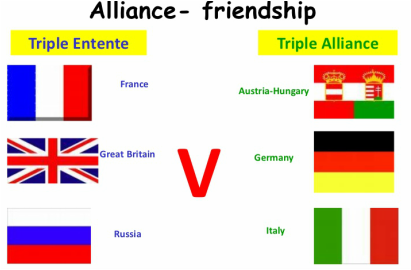
\includegraphics[width=10cm]{./img/tripleEntente.png}\end{center}
The Triple Entente refers to the understanding linking the Russian Empire, the French Third Republic, and United Kingdom of Great Britain and Ireland after the signing of the Anglo-Russian Entente on 31 August 1907. The understanding between the three powers, supplemented by agreements with Japan and Portugal, was a powerful counterweight to the Triple Alliance of Germany, Austria-Hungary, and Italy.

However, Italy did not side with Germany and Austria during World War I and joined the Entente instead in the Treaty of London (1915).

Historians continue to debate the importance of the alliance system as one of the causes of World War I. At the start of World War I in 1914, all three Triple Entente members entered it as Allied Powers against the Central Powers: Germany and Austria-Hungary.

However, the Triple Entente, unlike the Triple Alliance or the Franco-Russian Alliance, was not an alliance of mutual defense. Thus, Britain felt free to make its own foreign policy decisions in the 1914 July Crisis.

\chapter{1912}
\section{14-15 April}
\subsection{Sinking of the RMS Titanic}

\chapter{1914}
\section{June 28}
\subsection{Assassination of Franz Ferdinand}
\vspace{2mm}\begin{center}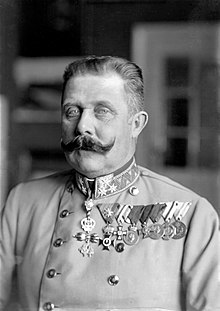
\includegraphics[width=8cm]{./img/ferdinand.jpg}\end{center}
The assassination of Archduke Franz Ferdinand of Austria, heir presumptive to the Austro-Hungarian throne, and his wife Sophie, Duchess of Hohenberg, occurred on 28 June 1914 in Sarajevo when they were mortally wounded by Gavrilo Princip.

\section{July 28}
\subsection{Austria-Hungary declares war on Serbia (World War I begins)}
\vspace{2mm}\begin{center}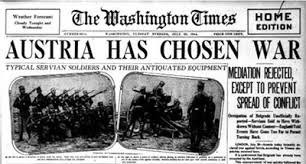
\includegraphics[width=10cm]{./img/austriaWarSerbia.jpg}\end{center}
On July 28, 1914, one month to the day after Archduke Franz Ferdinand of Austria and his wife were killed by a Serbian nationalist in Sarajevo, Austria-Hungary declares war on Serbia, effectively beginning the First World War

\section{July 31}
\subsection{Russia mobilizes its army in defense of Serbia}
\vspace{2mm}\begin{center}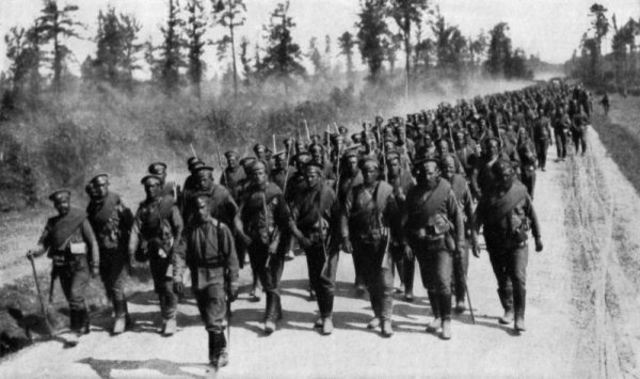
\includegraphics[width=10cm]{./img/russianTroops.jpg}\end{center}
July 31, 1914 - Reacting to the Austrian attack on Serbia, Russia begins full mobilization of its troops. Germany demands that it stop. August 1, 1914 - Germany declares war on Russia.

\section{August 01-03}
\subsection{Germany declares war on Russia and France}
\vspace{2mm}\begin{center}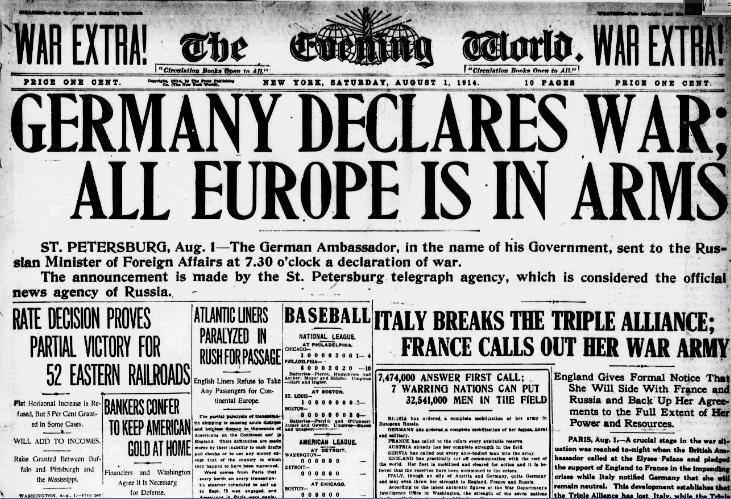
\includegraphics[width=10cm]{./img/germanyWarDeclaration.jpg}\end{center}
August 1, 1914 - Germany declares war on Russia. France and Belgium begin full mobilization. August 3, 1914 - Germany declares war on France, and invades neutral Belgium. Britain then sends an ultimatum, rejected by the Germans, to withdraw from Belgium.

\section{August 04}
\subsection{Germany invades neutral Belgium}
\vspace{2mm}\begin{center}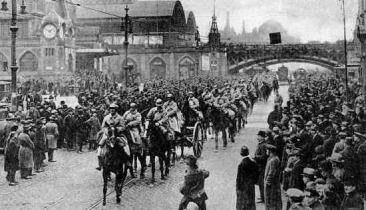
\includegraphics[width=12cm]{./img/germanyInBelgium.jpg}\end{center}
The German invasion of Belgium was a military campaign which began on 4 August 1914. Earlier, on 24 July, the Belgian government had announced that if war came it would uphold its historic neutrality. The Belgian government mobilised its armed forces on 31 July and a state of heightened alert (Kriegsgefahr) was proclaimed in Germany. On 2 August, the German government sent an ultimatum to Belgium, demanding passage through the country and German forces invaded Luxembourg. Two days later, the Belgian Government refused the demands and the British Government guaranteed military support to Belgium. The German government declared war on Belgium on 4 August, troops crossed the border and began the Battle of Liège.

\section{August 05}
\subsection{Battle of Liège}
\vspace{2mm}\begin{center}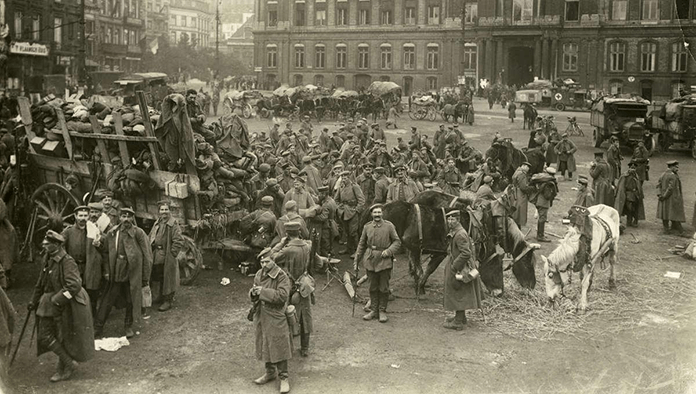
\includegraphics[width=12cm]{./img/battleOfLiege.png}\end{center}
The Battle of Liège (French: Bataille de Liège) was the opening engagement of the German invasion of Belgium and the first battle of the First World War. The attack on Liège, a town protected by the Fortified position of Liège, a ring fortress built from the late 1880s to the early 1890s, began on 5 August 1914 and lasted until 16 August, when the last fort surrendered. The siege of Liège may have delayed the German invasion of France by 4–5 days. Railways in the Meuse river valley needed by the German armies in eastern Belgium were closed for the duration of the siege and German troops did not appear in strength before the Fortified Position of Namur at the confluence of the Sambre and Meuse rivers until 20 August.

\section{August 15-24}
\subsection{Battle of Cer}
\vspace{2mm}\begin{center}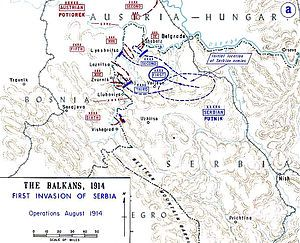
\includegraphics[width=8cm]{./img/battleOfCer.jpg}\end{center}
The Battle of Cer was a military campaign fought between Austria-Hungary and Serbia in August 1914 during the early stages of the Serbian Campaign of the First World War. It took place around Cer Mountain and several surrounding villages, as well as the town of Šabac.

The battle, part of the first Austro-Hungarian invasion of Serbia, began on the night of 15 August when elements of the Serbian 1st Combined Division encountered Austro-Hungarian outposts that had been established on the slopes of Cer Mountain earlier in the invasion. The clashes that followed escalated into a battle for control over several towns and villages near the mountain, especially Šabac. On 19 August, the morale of the Austro-Hungarians collapsed and thousands of soldiers retreated back into Austria-Hungary, many of them drowning in the Drina River as they fled in panic. On 24 August the Serbs re-entered Šabac, marking the end of the battle. Serbian casualties after nearly ten days of fighting were 3,000–5,000 killed and 15,000 wounded. Those of the Austro-Hungarians were significantly higher, with 6,000–10,000 soldiers killed, 30,000 wounded and 4,500 taken as prisoners of war. The Serb victory over the Austro-Hungarians marked the first Allied victory over the Central Powers in the First World War, and the first aerial dogfight of the war took place during the battle.

\section{August-September}
\subsection{Battle of Galicia}
\vspace{2mm}\begin{center}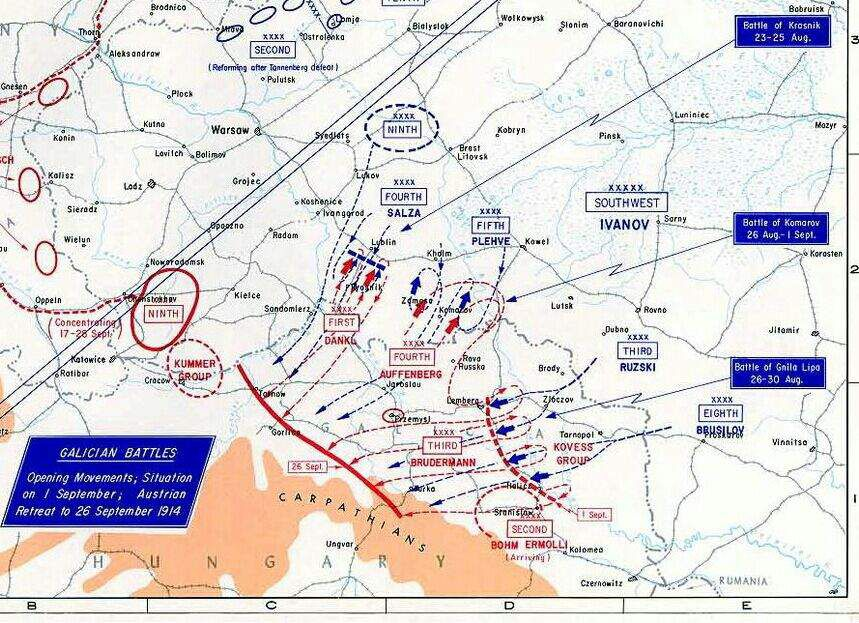
\includegraphics[width=10cm]{./img/battleOfGalicia.jpg}\end{center}
The Battle of Galicia, also known as the Battle of Lemberg, was a major battle between Russia and Austria-Hungary during the early stages of World War I in 1914. In the course of the battle, the Austro-Hungarian armies were severely defeated and forced out of Galicia, while the Russians captured Lemberg and, for approximately nine months, ruled Eastern Galicia until their defeat at Gorlice and Tarnów.

\subsection{Battle of Frontiers}
\vspace{2mm}\begin{center}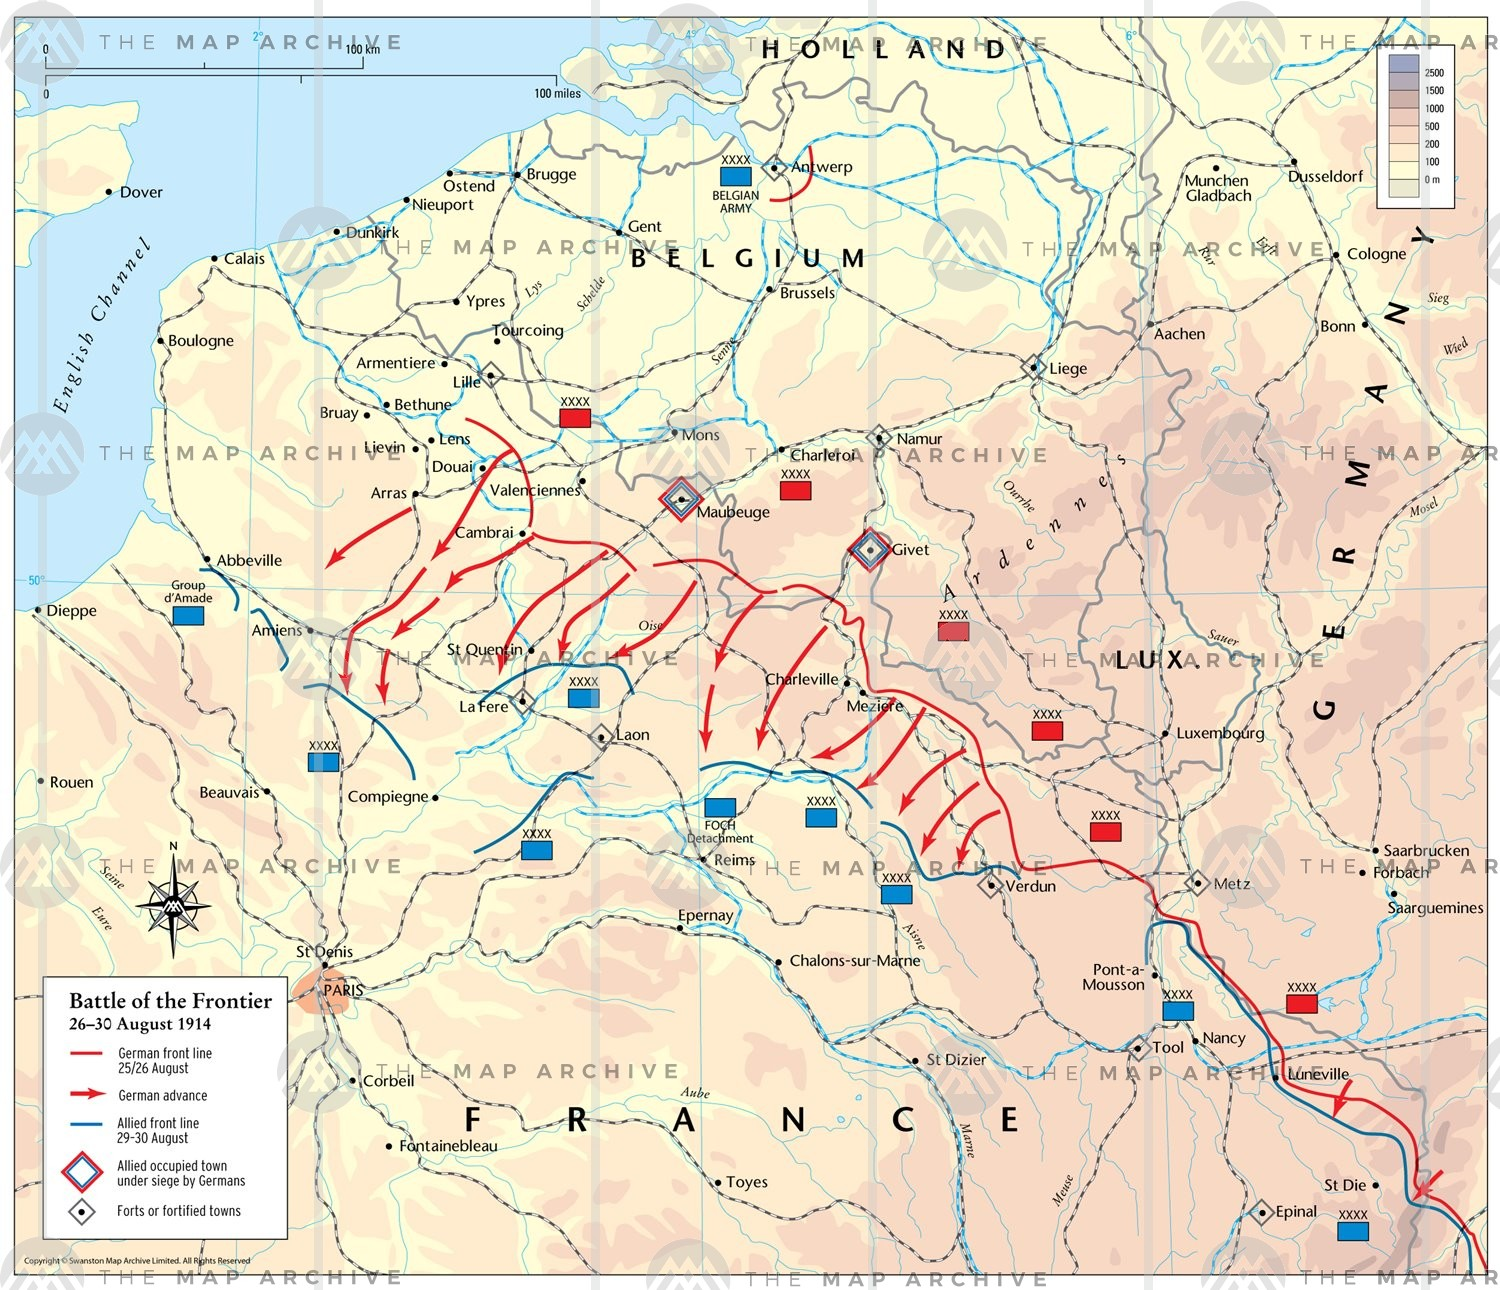
\includegraphics[width=10cm]{./img/battleOfFrontier.jpg}\end{center}
The Battle of the Frontiers (Dutch: Slag der Grenzen; French: Bataille des Frontières; German: Grenzschlachten) was a series of battles fought along the eastern frontier of France and in southern Belgium, shortly after the outbreak of the First World War. The battles resolved the military strategies of the French Chief of Staff General Joseph Joffre with Plan XVII and an offensive interpretation of the German Aufmarsch II deployment plan by Helmuth von Moltke the Younger. The German concentration on the right (northern) flank, to wheel through Belgium and attack the French in the rear, was delayed by the movement of French Fifth Army (General Charles Lanrezac) towards the north-west to intercept them and the presence of the British Expeditionary Force (BEF) on his left flank. The Franco-British were driven back by the Germans, who were able to invade northern France. French and British rearguard actions delayed the German advance, allowing the French time to transfer forces on the eastern frontier to the west to defend Paris, resulting in the First Battle of the Marne.

\section{December 25}
\subsection{The Christmas truce}
\vspace{2mm}\begin{center}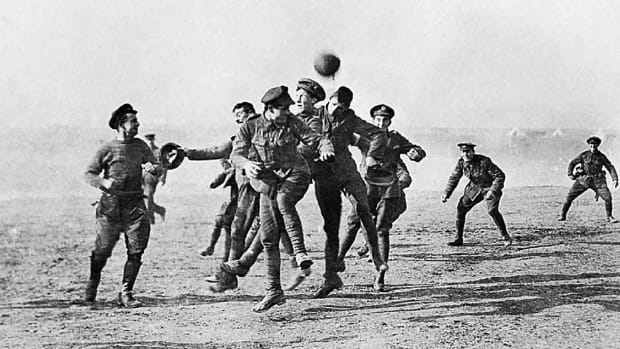
\includegraphics[width=10cm]{./img/christmasTruce.jpg}\end{center}
The Christmas truce occurred during the relatively early period of the war (month 5 of 51). Hostilities had entered somewhat of a lull as leadership on both sides reconsidered their strategies following the stalemate of the Race to the Sea and the indecisive result of the First Battle of Ypres. In the week leading up to the 25th, French, German, and British soldiers crossed trenches to exchange seasonal greetings and talk. In some areas, men from both sides ventured into no man's land on Christmas Eve and Christmas Day to mingle and exchange food and souvenirs. There were joint burial ceremonies and prisoner swaps, while several meetings ended in carol-singing. Men played games of football with one another, giving one of the most memorable images of the truce. Peaceful behavior was not ubiquitous; fighting continued in some sectors, while in others the sides settled on little more than arrangements to recover bodies.

\chapter{1917}
\section{February 23 - March 3}
\subsection{Russian Revolution (February)}
\section{October 25-26}
\subsection{Russian Revolution (October)}


\chapter{1918}
\section{January}
\subsection{Spanish flu}

\section{November 11}
\subsection{World War I ends}

\section{October 29}
\subsection{The German Revolution}
\vspace{2mm}\begin{center}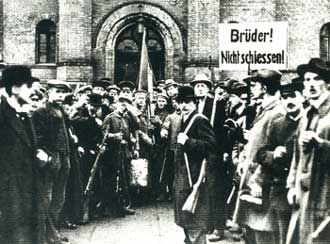
\includegraphics[width=10cm]{./img/germanRevolution.jpg}\end{center}
The German Revolution or November Revolution (German: Novemberrevolution) was a civil conflict in the German Empire at the end of the First World War that resulted in the replacement of the German federal constitutional monarchy with a democratic parliamentary republic that later became known as the Weimar Republic. The revolutionary period lasted from November 1918 until the adoption in August 1919 of the Weimar Constitution.

\chapter{1919}
\section{June 28}
\subsection{Treaty of Versailles}

\chapter{1929}
\section{October 24 "Black Thursday"}
\subsection{The Wall Street Crash}
\vspace{2mm}\begin{center}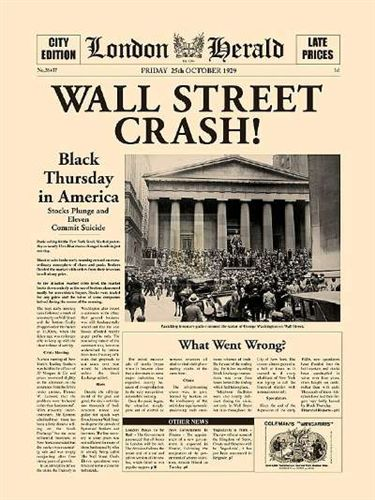
\includegraphics[width=8cm]{./img/wallStreetCrash.jpg}\end{center}
The Wall Street Crash of 1929, also known as the Stock Market Crash of 1929 or the Great Crash, is the stock market crash that occurred in late October, 1929. It started on October 24 ("Black Thursday") and continued until October 29, 1929 ("Black Tuesday"), when share prices on the New York Stock Exchange collapsed.

\chapter{1930}
\section{July 13-30}
\subsection{FIFA World Cup}
\vspace{2mm}\begin{center}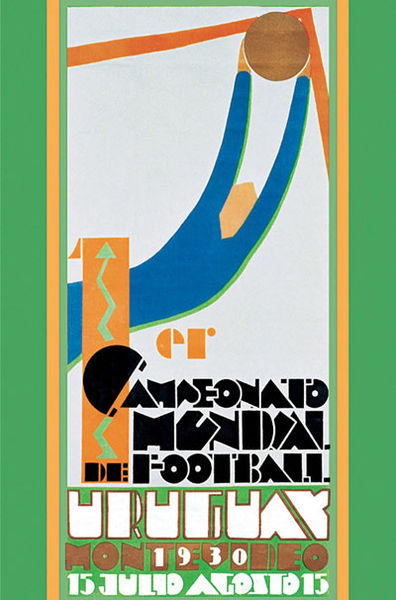
\includegraphics[width=5cm]{./img/fifa1930.jpg}\end{center}
The 1930 FIFA World Cup was the inaugural FIFA World Cup, the world championship for men's national association football teams. It took place in Uruguay from 13 to 30 July 1930. FIFA, football's international governing body, selected Uruguay as host nation, as the country would be celebrating the centenary of its first constitution, and the Uruguay national football team had successfully retained their football title at the 1928 Summer Olympics. All matches were played in the Uruguayan capital, Montevideo, the majority at the Estadio Centenario, which was built for the tournament.

\chapter{1933}
\section{December 26}
\subsection{Nissan if founded}
\vspace{2mm}\begin{center}
\includegraphics[width=8cm]{./img/nissan.jpg}\end{center}
Nissan Motor Co., Ltd. is a Japanese multinational automobile manufacturer headquartered in Nishi-ku, Yokohama. The company sells its cars under the Nissan, Infiniti, and Datsun brands with in-house performance tuning products labelled Nismo. The company traces its name to the Nissan zaibatsu, now called Nissan Group.

\chapter{1939}
\section{September 1}
\subsection{World War II begins}

\chapter{1940}
\section{May 15}
\subsection{McDonald's is founded \protect\footnote{Movie/Documentary: The Founder (2016)}}
\vspace{2mm}\begin{center}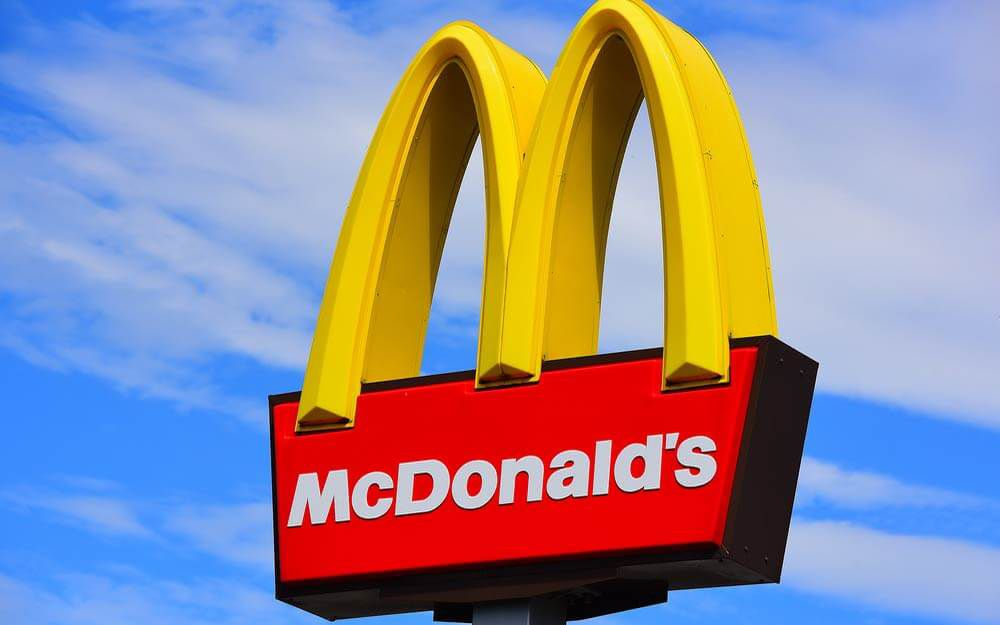
\includegraphics[width=12cm]{./img/mcdonalds.jpg}\end{center}
McDonald's is an American fast food company, founded in 1940 as a restaurant operated by Richard and Maurice McDonald, in San Bernardino, California, United States. They rechristened their business as a hamburger stand, and later turned the company into a franchise, with the Golden Arches logo being introduced in 1953 at a location in Phoenix, Arizona. In 1955, Ray Kroc, a businessman, joined the company as a franchise agent and proceeded to purchase the chain from the McDonald brothers. McDonald's had its original headquarters in Oak Brook, Illinois, but moved its global headquarters to Chicago in early 2018.

\chapter{1942}
\section{January 8}
\subsection{Birth of Stephen Hawking}
\vspace{2mm}\begin{center}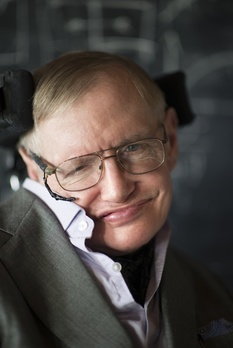
\includegraphics[width=5cm]{./img/stephenhawking.jpg}\end{center}
Stephen William Hawking (8 January 1942 – 14 March 2018) was an English theoretical physicist, cosmologist, and author, who was director of research at the Centre for Theoretical Cosmology at the University of Cambridge at the time of his death. He was the Lucasian Professor of Mathematics at the University of Cambridge between 1979 and 2009.\\
His scientific works included a collaboration with Roger Penrose on gravitational singularity theorems in the framework of general relativity and the theoretical prediction that black holes emit radiation, often called Hawking radiation. Hawking was the first to set out a theory of cosmology explained by a union of the general theory of relativity and quantum mechanics. He was a vigorous supporter of the many-worlds interpretation of quantum mechanics.

\chapter{1945}
\section{September 2}
\subsection{World War II ends}
\vspace{2mm}\begin{center}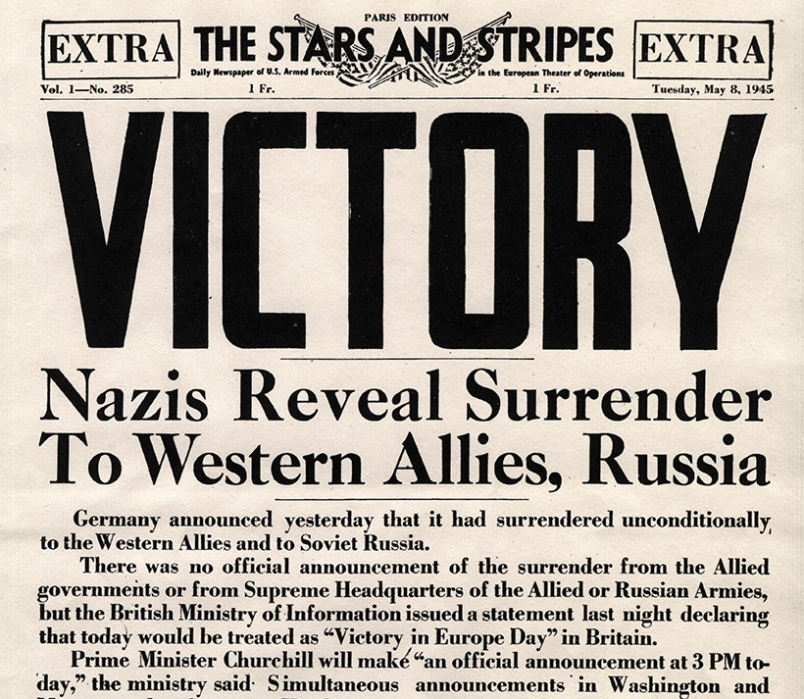
\includegraphics[width=8cm]{./img/endww2.jpg}\end{center}
The war in Europe concluded with an invasion of Germany by the Western Allies and the Soviet Union, culminating in the capture of Berlin by Soviet troops, the suicide of Adolf Hitler and the German unconditional surrender on 8 May 1945. Following the Potsdam Declaration by the Allies on 26 July 1945 and the refusal of Japan to surrender under its terms, the United States dropped atomic bombs on the Japanese cities of Hiroshima and Nagasaki on 6 and 9 August respectively. With an invasion of the Japanese archipelago imminent, the possibility of additional atomic bombings, the Soviet entry into the war against Japan and its invasion of Manchuria, Japan announced its intention to surrender on 15 August 1945, cementing total victory in Asia for the Allies. Tribunals were set up by fiat by the Allies and war crimes trials were conducted in the wake of the war both against the Germans and the Japanese.

\chapter{1946}
\section{May 7}
\subsection{Sony is founded}
\vspace{2mm}\begin{center}
\includegraphics[width=10cm]{./img/sonylogo.png}\end{center}
Sony began in the wake of World War II. In 1946, Masaru Ibuka started an electronics shop in a department store building in Tokyo. The company started with a capital of 190,000 Yen and a total of eight employees. In May 1946, Ibuka was joined by Akio Morita to establish a company called Tokyo Tsushin Kogyo (Tōkyō Tsūshin Kōgyō) (Tokyo Telecommunications Engineering Corporation). The company built Japan's first tape recorder, called the Type-G. In 1958, the company changed its name to "Sony"

\chapter{1947}
\section{August 14}
\subsection{The birth of Pakistan \protect\footnote{Movie/Documentary: Gandhi (1982)}}
\vspace{2mm}\begin{center}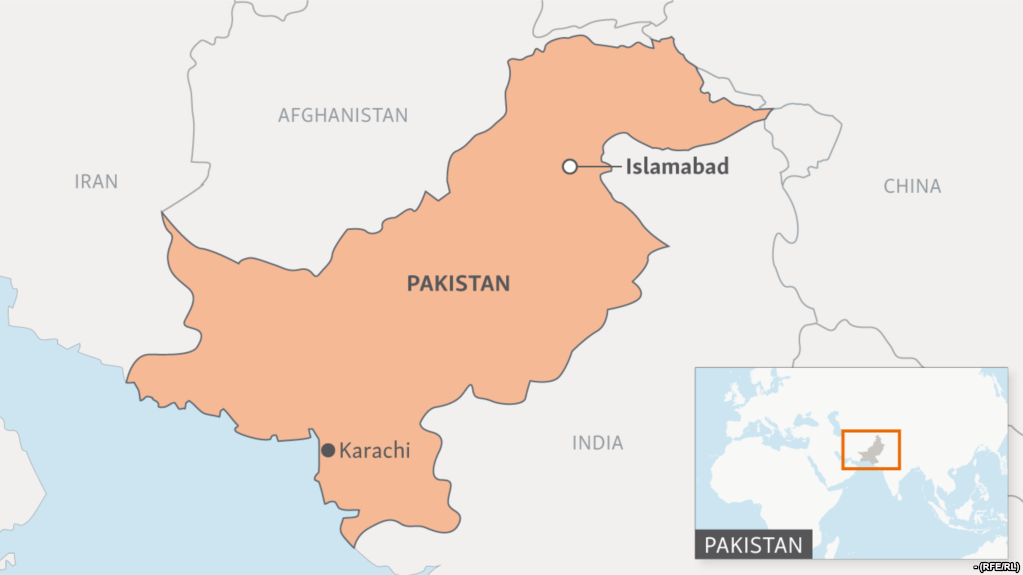
\includegraphics[width=10cm]{./img/pakistan.png}\end{center}
Pakistan, or the Islamic Republic of Pakistan as it is officially known, is a relatively young country, emerging on 14 August 1947. On 14 August 1947 the new independent nation of Pakistan was born, followed closely by India's independence on 15 August 1947.

\section{August 15}
\subsection{Independence of India \protect\footnote{Movie/Documentary: Gandhi (1982)}}
\vspace{2mm}\begin{center}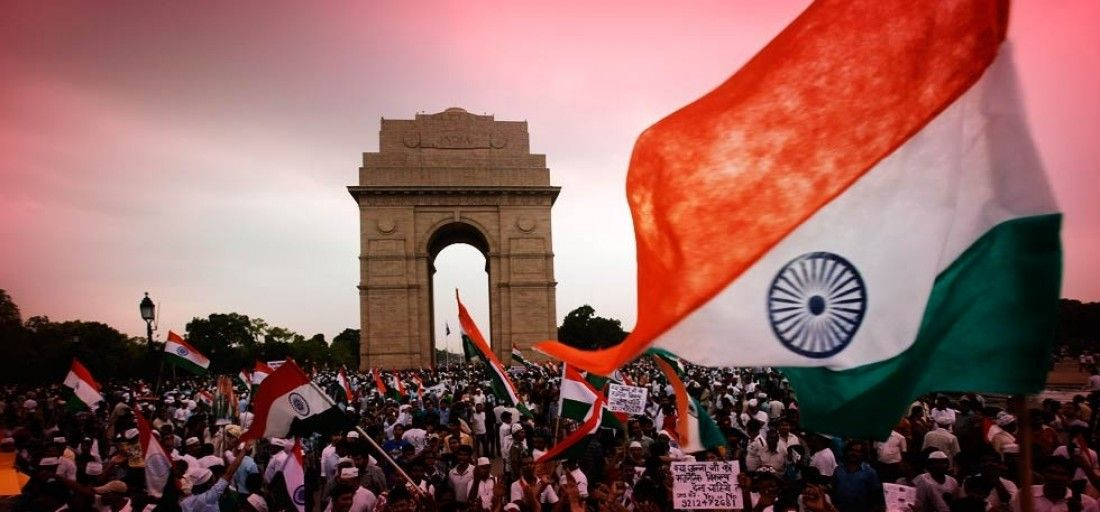
\includegraphics[width=12cm]{./img/independenceIndia.jpg}\end{center}
European traders had established outposts in the Indian subcontinent by the 17th century. Through overwhelming military strength, the British East India company subdued local kingdoms and established themselves as the dominant force by the 18th century. Following the First War of Independence of 1857, the Government of India Act 1858 led the British Crown to assume direct control of India. In the decades following, civic society gradually emerged across India, most notably the Indian National Congress Party, formed in 1885. The period after World War I was marked by British reforms such as the Montagu–Chelmsford Reforms, but it also witnessed the enactment of the repressive Rowlatt Act and calls for self-rule by Indian activists. The discontent of this period crystallised into nationwide non-violent movements of non-cooperation and civil disobedience, led by Mohandas Karamchand Gandhi

During the 1930s, the reform was gradually legislated by the British; Congress won victories in the resulting elections. The next decade was beset with political turmoil: Indian participation in World War II, the Congress' final push for non-cooperation, and an upsurge of Muslim nationalism led by the All-India Muslim League. The escalating political tension was capped by Independence in 1947. The jubilation was tempered by the bloody partition of the subcontinent into India and Pakistan.
%\subsubsection{Movie/documentary: Gandhi (1982)}

\chapter{1948}
\section{January 30}
\subsection{Assassination of Mahatma Gandhi\protect\footnote{Movie/Documentary: Gandhi (1982)}}
\vspace{2mm}\begin{center}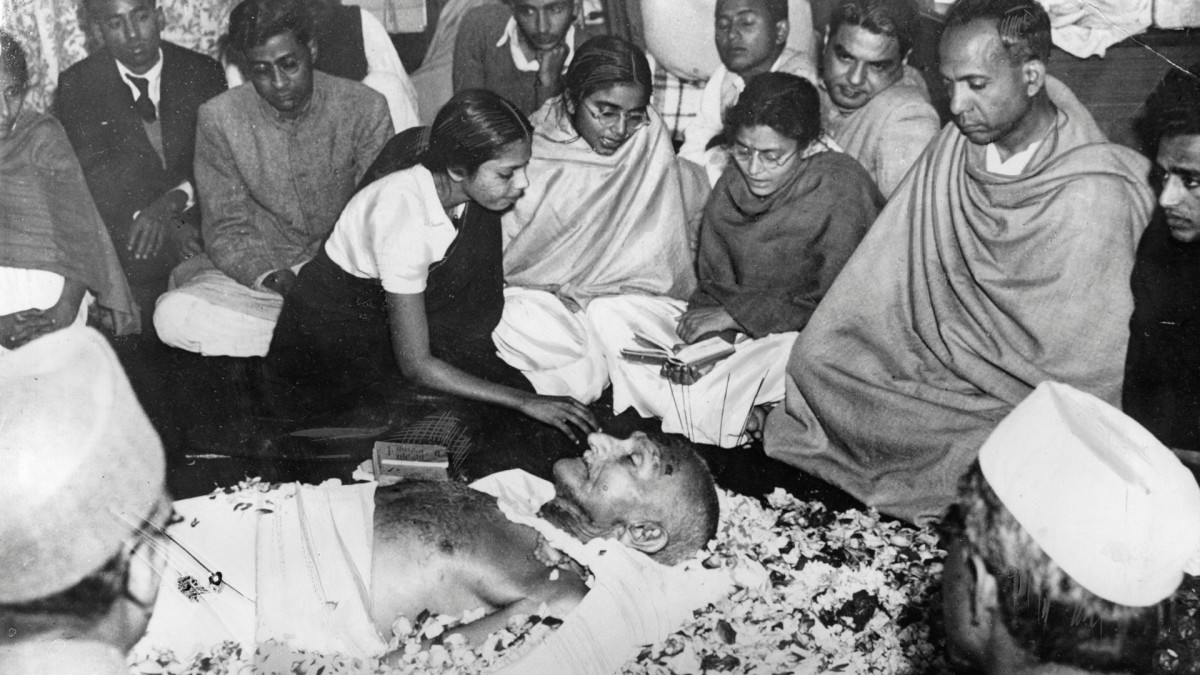
\includegraphics[width=12cm]{./img/gandhiDead.jpg}\end{center}
Mahatma Gandhi was assassinated on 30 January 1948 in the compound of Birla House (now Gandhi Smriti), a large mansion. His assassin was Nathuram Vinayak Godse, a freedom fighter, advocate of Indian nationalism, a member of the political party the Hindu Mahasabha, and a past member of the Rashtriya Swayamsevak Sangh (RSS), which he left in 1940 to form an armed organization. Godse had planned the assassination.

Gandhi had just walked up the low steps to the raised lawn behind Birla House where he conducted his multi-faith prayer meetings every evening. Godse stepped out from the crowd flanking the path leading to the dais and into Gandhi's path, firing three bullets at point-blank range. Gandhi instantly fell to the ground. Gandhi was carried back to his room in Birla House from where a representative emerged some time later to announce that he had died.

\chapter{1954}
\section{July 29}
\subsection{"LOTR: The Fellowship of the Ring"\protect\footnote{The Lord of the Rings: The Fellowship of the Ring (2001)} published}
\vspace{2mm}\begin{center}\includegraphics[width=5cm]{./img/lotrbook1.jpg}\end{center}
The Fellowship of the Ring is the first of three volumes of the epic novel The Lord of the Rings by the English author J. R. R. Tolkien. It is followed by The Two Towers and The Return of the King. It takes place in the fictional universe of Middle-earth. It was originally published on 29 July 1954 in the United Kingdom.

The volume consists of a foreword, in which the author discusses his writing of The Lord of the Rings, a prologue titled "Concerning Hobbits, and other matters", and the main narrative in Book I and Book II.

\chapter{1957}
\section{}
\subsection{The beginning of space age}
\vspace{2mm}\begin{center}\includegraphics[width=10cm]{./img/spaceage.jpg}\end{center}
The Space Age is a time period encompassing the activities related to the Space Race, space exploration, space technology, and the cultural developments influenced by these events. The Space Age is generally considered to have begun with Sputnik (1957).

\chapter{1962}
\section{November 3}
\subsection{Birth of Gabe Newell}
\vspace{2mm}\begin{center}\includegraphics[width=10cm]{./img/gaben.jpg}\end{center}
Gabe Logan Newell (born November 3, 1962), commonly known by his nickname Gaben, is an American computer programmer and businessman best known as the co-founder of the video game development and digital distribution company Valve Corporation. Born in Colorado, he attended Harvard University in the early 1980s, but dropped out and soon went to work for the American technology company Microsoft, where he spent the next decade working as a producer for some of their early Windows operating systems. \\

During his time at Microsoft, Newell, along with fellow co-worker Mike Harrington, were impressed by computer games that were being released in the mid-1990s, such as id Software's Doom and Quake. Fully convinced that video games were the future of entertainment, and intrigued by the prospect of having his own game development studio, Newell, along with Harrington, left Microsoft in 1996 to found Valve, of which he remains president.

\chapter{1969}
\section{July 20}
\subsection{Landing on The Moon (Apollo 11)}
\vspace{2mm}\begin{center}\includegraphics[width=12cm]{./img/apollo11.jpg}\end{center}
Apollo 11 was the spaceflight that landed the first two people on the Moon. Commander Neil Armstrong and Lunar Module Pilot Buzz Aldrin, both American, landed the lunar module Eagle on July 20, 1969, at 20:17 UTC. Armstrong became the first person to step onto the lunar surface six hours after landing on July 21 at 02:56:15 UTC; Aldrin joined him about 20 minutes later. They spent about two and a quarter hours together outside the spacecraft, and collected 47.5 pounds (21.5 kg) of lunar material to bring back to Earth. Command Module Pilot Michael Collins piloted the command module Columbia alone in lunar orbit while they were on the Moon's surface. Armstrong and Aldrin spent 21.5 hours on the lunar surface before rejoining Columbia in lunar orbit.

\chapter{1975}
\section{November}
\subsection{Moroccan Green March}
\vspace{2mm}\begin{center}\includegraphics[width=12cm]{./img/greenmarch.jpg}\end{center}
The Green March was a strategic mass demonstration in November 1975, coordinated by the Moroccan government, to force Spain to hand over the disputed, autonomous semi-metropolitan province of Spanish Sahara to Morocco. The demonstration of some 350,000 Moroccans advanced several kilometres into the Western Sahara territory, escorted by nearly 20,000 Moroccan troops, and meeting very little response by the Sahrawi Polisario Front. Nevertheless, the events quickly escalated into a fully waged war between Morocco and the militias of the Polisario, the Western Sahara War, which would last for 16 years. Morocco later gained control over most of the former Spanish Sahara, which it continues to hold.

\chapter{1977}
\section{August 20 to September 05}
\subsection{Beginning of the Voyager program \protect\footnote{Documentary: The Farthest (2017)}}
\vspace{2mm}\begin{center}\includegraphics[width=12cm]{./img/voyagerProgram.jpg}\end{center}
The Voyager program is an American scientific program that employs two robotic probes, Voyager 1 and Voyager 2, to study the outer Solar System. The probes were launched in 1977 to take advantage of a favorable alignment of Jupiter, Saturn, Uranus and Neptune. Although their original mission was to study only the planetary systems of Jupiter and Saturn, Voyager 2 continued on to Uranus and Neptune. The Voyagers now explore the outer boundary of the heliosphere in interstellar space; their mission has been extended three times and they continue to transmit useful scientific data. Neither Uranus nor Neptune has been visited by a probe other than Voyager 2.

\chapter{1979}
\section{December 25}
\subsection{Egypt begins major restoration of the Sphinx}
\vspace{2mm}\begin{center}\includegraphics[width=6.5cm]{./img/sphinxRestoration.jpg}\end{center}
The Great Sphinx of Giza, guardian of the Pyramids, is being shored up with limestone blocks in the most extensive repairs since the Romans worked on it more than 2,000 years ago.
Chemical processes caused by wind, water and the sun have eroded the Sphinx since it was chiseled out of bedrock 4,600 years ago. Some Egyptologists say the erosion, if not stopped, could eventually cause the head to topple. But they are reluctant to predict when.
Egyptian stonemasons arrived at the Sphinx recently, set up scaffolding along its right flank and crawled across the body to prepare for attaching a sort of stone corset.

\chapter{1983}
\section{November 10}
\subsection{Windows announced}
\vspace{2mm}\begin{center}\includegraphics[width=7cm]{./img/windows.png}\end{center}
Microsoft Windows was announced by Bill Gates on November 10, 1983. Microsoft introduced Windows as a graphical user interface for MS-DOS, which had been introduced a couple of years earlier. In the 1990s, the product line evolved from an operating environment into a fully complete, modern operating system over two lines of development, each with their own separate codebase.\\
The first versions of Windows (1.0 through to 3.11) were graphical shells that run from MS-DOS; later on, Windows 95, though still being based on MS-DOS, was its own operating system, using a 16-bit DOS-based kernel and a 32-bit user space. Windows 95 introduced many features that have been part of the product ever since, including the Start menu, the taskbar, and Windows Explorer (renamed File Explorer in Windows 8). In 1997, Microsoft released Internet Explorer 4 which included the (at the time) controversial Windows Desktop Update. It aimed to integrate Internet Explorer and the web into the user interface and also brought many new features into Windows, such as the ability to display JPEG images as the desktop wallpaper and single window navigation in Windows Explorer.
\begin{comment}
In 1998, Microsoft released Windows 98, which also included the Windows Desktop Update and Internet Explorer 4 by default. The inclusion of Internet Explorer 4 and the Desktop Update led to an anti-trust case in the United States. Windows 98 also includes plug and play, which allows devices to work when plugged in without requiring a system reboot or manual configuration, and USB support out of the box. Windows ME, the last DOS-based version of Windows, was aimed at consumers and released in 2000. It introduced System Restore, Help and Support Center, updated versions of the Disk Defragmenter and other system tools.
\end{comment}

\chapter{1986}
\section{April 25-26}
\subsection{Chernobyl disaster}
\vspace{2mm}\begin{center}\includegraphics[width=8cm]{./img/chernobyl.jpg}\end{center}
The Chernobyl disaster, also referred to as the Chernobyl accident, was a catastrophic nuclear accident. It occurred on 25–26 April 1986 in the No. 4 light water graphite moderated reactor at the Chernobyl Nuclear Power Plant near the now-abandoned town of Pripyat, in northern Ukrainian Soviet Socialist Republic, Soviet Union, approximately 104 km (65 mi) north of Kiev.

The event occurred during a late-night safety test which simulated a station blackout power-failure, in the course of which safety systems were intentionally turned off. A combination of inherent reactor design flaws and the reactor operators arranging the core in a manner contrary to the checklist for the test, eventually resulted in uncontrolled reaction conditions. Water flashed into steam generating a destructive steam explosion and a subsequent open-air graphite fire. This fire produced considerable updrafts for about nine days. These lofted plumes of fission products into the atmosphere. The estimated radioactive inventory that was released during this very hot fire phase approximately equaled in magnitude the airborne fission products released in the initial destructive explosion. This radioactive material precipitated onto parts of the western USSR and Europe.

\chapter{1989}
\section{November 09}
\subsection{Fall of the Berlin Wall}
\vspace{2mm}\begin{center}\includegraphics[width=10cm]{./img/fallBerlinWall.jpg}\end{center}
On November 9, 1989, as the Cold War began to thaw across Eastern Europe, the spokesman for East Berlin’s Communist Party announced a change in his city’s relations with the West. Starting at midnight that day, he said, citizens of the GDR were free to cross the country’s borders. East and West Berliners flocked to the wall, drinking beer and champagne and chanting “Tor auf!” (“Open the gate!”). At midnight, they flooded through the checkpoints.

More than 2 million people from East Berlin visited West Berlin that weekend to participate in a celebration that was, one journalist wrote, “the greatest street party in the history of the world.” People used hammers and picks to knock away chunks of the wall–they became known as “mauerspechte,” or “wall woodpeckers”—while cranes and bulldozers pulled down section after section. Soon the wall was gone and Berlin was united for the first time since 1945. “Only today,” one Berliner spray-painted on a piece of the wall, “is the war really over.”

\section{?}
\subsection{Tim Berners-Lee invents the World Wide Web \protect\footnote{Lo and Behold: Reveries of the Connected World (2016)}}
\vspace{2mm}\begin{center}\includegraphics[width=10cm]{./img/www.jpg}\end{center}
The World Wide Web was invented by English scientist Tim Berners-Lee in 1989. He wrote the first web browser in 1990 while employed at CERN in Switzerland. Web pages are primarily text documents formatted and annotated with Hypertext Markup Language (HTML).

\chapter{1990}
\section{April 24}
\subsection{Launch of the Hubble Space Telescope}
\vspace{2mm}\begin{center}\includegraphics[width=6cm]{./img/hubble.jpg}\end{center}
The Hubble Space Telescope (HST) is a space telescope that was launched into low Earth orbit in 1990 and remains in operation. Although not the first space telescope, Hubble is one of the largest and most versatile and is well known as both a vital research tool and a public relations boon for astronomy. The HST is named after the astronomer Edwin Hubble and is one of NASA's Great Observatories, along with the Compton Gamma Ray Observatory, the Chandra X-ray Observatory and the Spitzer Space Telescope.

\section{August 2}
\subsection{Invasion of Kuwait}
\vspace{2mm}\begin{center}\includegraphics[width=10cm]{./img/iraqKuwaitWar.jpg}\end{center}
The Invasion of Kuwait on 2 August 1990 was a two-day operation conducted by Iraq against the neighboring state of Kuwait, which resulted in the seven-month-long Iraqi occupation of the country. This invasion and Iraq's subsequent refusal to withdraw from Kuwait by a deadline mandated by the United Nations[8] led to military intervention by a United Nations-authorized coalition of forces led by the United States. These events came to be known as the first Gulf War and resulted in the expulsion of Iraqi forces from Kuwait and the Iraqis setting 600 Kuwaiti oil wells on fire during their retreat.

\chapter{1991}
\section{August 06}
\subsection{First Website is put online and available to the public}

\section{December 26}
\subsection{Dissolution of the Soviet Union}
\vspace{2mm}\begin{center}\includegraphics[width=10cm]{./img/ussr.jpg}\end{center}
The dissolution of the Soviet Union occurred on 26 December 1991, officially granting self-governing independence to the Republics of the Union of Soviet Socialist Republics (USSR). It was a result of the declaration number 142-H of the Supreme Soviet of the Soviet Union.

\chapter{1992}
\section{February 07}
\subsection{Maastricht Treaty creates the European Union}
\vspace{2mm}\begin{center}\includegraphics[width=12cm]{./img/maastrichtTreaty.jpg}\end{center}
The Maastricht Treaty (officially the Treaty on European Union) was signed on 7 February 1992 by the members of the European Community in Maastricht, Netherlands to further European integration. On 9–10 December 1991, the same city hosted the European Council which drafted the treaty. The treaty founded the European Union and established its pillar structure which stayed in place until the Lisbon Treaty came into force in 2009. The treaty also greatly expanded the competences of the EEC/EU and led to the creation of the single European currency, the euro.

\section{February 22}
\subsection{The first extra-solar planet is confirmed}
\vspace{2mm}\begin{center}\includegraphics[width=10cm]{./img/PSR_B1257_12_C.jpg}\end{center}
The first suspected scientific detection of an exoplanet occurred in 1988. Shortly afterwards, the first confirmed detection came in 1992, with the discovery of several terrestrial-mass planets orbiting the pulsar PSR B1257+12

\chapter{1994}
\section{March 10}
\subsection{Election of Nelson Mandela}
\vspace{2mm}\begin{center}\includegraphics[width=4cm]{./img/mandela.jpg}\end{center}
The African National Congress won 62\% of the votes in the election, and Mandela, as leader of the ANC, was inaugurated on 10 May 1994 as the country's first black President, with the National Party's F.W. de Klerk as his first deputy and Thabo Mbeki as the second in the Government of National Unity.

\chapter{1995}
\section{August 16}
\subsection{First release of Internet Explorer}
\vspace{2mm}\begin{center}\includegraphics[width=12cm]{./img/internetExplorer.jpg}\end{center}
Microsoft originally released Internet Explorer 1.0 in August 1995 in two packages: at retail in Microsoft Plus!

\chapter{1996}
\section{July 05}
\subsection{The first successful cloned mammal: Dolly the sheep}
\vspace{2mm}\begin{center}\includegraphics[width=9cm]{./img/dollySheep.jpg}\end{center}
Dolly was cloned by Keith Campbell, Ian Wilmut and colleagues at the Roslin Institute, part of the University of Edinburgh, Scotland, and the biotechnology company PPL Therapeutics, based near Edinburgh. The funding for Dolly's cloning was provided by PPL Therapeutics and the Ministry of Agriculture. She was born on 5 July 1996 and died from a progressive lung disease five months before her seventh birthday (the disease was not considered related to her being a clone). She has been called "the world's most famous sheep" by sources including BBC News and Scientific American.

The cell used as the donor for the cloning of Dolly was taken from a mammary gland, and the production of a healthy clone therefore proved that a cell taken from a specific part of the body could recreate a whole individual. On Dolly's name, Wilmut stated "Dolly is derived from a mammary gland cell and we couldn't think of a more impressive pair of glands than Dolly Parton's".

\section{August 24}
\subsection{Valve Corp. is founded}
\vspace{2mm}\begin{center}\includegraphics[width=10cm]{./img/valve.jpg}\end{center}
Valve Corporation is an American video game developer, publisher and digital distribution company headquartered in Bellevue, Washington. It is the developer of the software distribution platform Steam and the Half-Life, Counter-Strike, Portal, Day of Defeat, Team Fortress, Left 4 Dead, and Dota 2 games.

Valve was founded in 1996 by former Microsoft employees Gabe Newell and Mike Harrington. Their debut product, the PC first-person shooter Half-Life, was released in 1998 to critical acclaim and commercial success, after which Harrington left the company. In 2003, Valve launched Steam, which accounted for around half of digital PC game sales by 2011. By 2012, Valve employed around 250 people and was reportedly worth over US\$3 billion, making it the most profitable company per employee in the United States. In 2015, Valve entered the game hardware market with the Steam Machine, a line of third-party built gaming PCs running Valve's SteamOS operating system.

\chapter{1998}
\section{September 04}
\subsection{Google is founded by Larry Page and Sergey Brin}
\vspace{2mm}\begin{center}\includegraphics[width=8cm]{./img/googlebeta.jpg}\end{center}
The Google company was officially launched in 1998 by Larry Page and Sergey Brin to market Google Search, which has become the most widely used web-based search engine. Page and Brin, students at Stanford University in California, developed a search algorithm – at first known as "BackRub" – in 1996. The search engine soon proved successful and the expanding company moved several times, finally settling at Mountain View in 2003. This marked a phase of rapid growth, with the company making its initial public offering in 2004 and quickly becoming one of the world's largest media companies. The company launched Google News in 2002, Gmail in 2004, Google Maps in 2005, Google Chrome in 2008, and the social network known as Google+ in 2011, in addition to many other products. In 2015, Google became the main subsidiary of the holding company Alphabet Inc.

\section{November 20}
\subsection{Construction of the ISS begins}
\vspace{2mm}\begin{center}\includegraphics[width=12cm]{./img/iss.jpg}\end{center}
Zarya, the first ISS module, was launched by a Proton rocket on November 20, 1998. The STS-88 shuttle mission followed two weeks after Zarya was launched, bringing Unity, the first of three node modules, and connecting it to Zarya.


								% 21ST CENTURY 


\part{21st century}
\chapter{2000}
\section{January 01}
\subsection{Beginning of the 3rd millennium}
\vspace{2mm}\begin{center}\includegraphics[width=12cm]{./img/fireworks.jpg}\end{center}
In contemporary history, the third millennium is a period of time that started on January 1, 2001, and will end on December 31, 3000 of the Gregorian calendar. It is distinct from the millennium known as the 2000s which began on January 1, 2000 and will end on December 31, 2999.

\chapter{2001}
\section{January 15}
\subsection{Wikipedia is founded}
\vspace{2mm}\begin{center}\includegraphics[width=8cm]{./img/wikipedia.png}\end{center}
Wikipedia began with its launch on 15 January 2001, two days after the domain was registered by Jimmy Wales and Larry Sanger. Its technological and conceptual underpinnings predate this; the earliest known proposal for an online encyclopedia was made by Rick Gates in 1993, but the concept of a free-as-in-freedom online encyclopedia (as distinct from mere open source) was proposed by Richard Stallman in December 2000

\section{September 11}
\subsection{9-11 Attacks}
\vspace{2mm}\begin{center}\includegraphics[width=12cm]{./img/9-11.jpg}\end{center}
The September 11 attacks (also referred to as 9/11) were a series of four coordinated terrorist attacks by the Islamic terrorist group al-Qaeda against the United States on the morning of Tuesday, September 11, 2001. The attacks killed 2,996 people, injured over 6,000 others, and caused at least \$ 10 billion in infrastructure and property damage. Additional people died of 9/11-related cancer and respiratory diseases in the months and years following the attacks.

\section{November 15}
\subsection{Xbox Introduced}
\vspace{2mm}\begin{center}\includegraphics[width=10cm]{./img/xbox1.jpg}\end{center}
Xbox is a video gaming brand created and owned by Microsoft of the United States. It represents a series of video game consoles developed by Microsoft, with three consoles released in the sixth, seventh and eighth generations, respectively. The brand also represents applications (games), streaming services, and an online service by the name of Xbox Live. The brand was first introduced in the United States in November 2001, with the launch of the original Xbox console.\\
The original device was the first video game console offered by an American company after the Atari Jaguar stopped sales in 1996. It reached over 24 million units sold as of May 2006. Microsoft's second console, the Xbox 360, was released in 2005 and has sold over 77.2 million consoles worldwide as of April 2013. The Xbox One has been released in 21 markets in total, with a Chinese release in September 2014. The head of Xbox is Phil Spencer, who succeeded former head Marc Whitten in late March 2014.

\chapter{2002}
\section{January 01}
\subsection{The Euro is introduced within the EU}
\vspace{2mm}\begin{center}\includegraphics[width=12cm]{./img/euro.jpg}\end{center}
The Euro is the new 'single currency' of the European Monetary Union, adopted on January 1, 1999 by 11 Member States. Greece became the 12th Member state to adopt the Euro on January 1, 2001. On January 1, 2002, these 12 countries officially introduced the Euro banknotes and coins as legal tender.

\chapter{2003}
\section{March 20}
\subsection{Beginning of the Iraq war}
\vspace{2mm}\begin{center}\includegraphics[width=10cm]{./img/iraqWar.jpg}\end{center}
The Iraq War was a protracted armed conflict that began in 2003 with the invasion of Iraq by a United States-led coalition that overthrew the government of Saddam Hussein. The conflict continued for much of the next decade as an insurgency emerged to oppose the occupying forces and the post-invasion Iraqi government. An estimated 151,000 to 600,000 or more Iraqis were killed in the first 3–4 years of conflict. The U.S. became re-involved in 2014 at the head of a new coalition; the insurgency and many dimensions of the civil armed conflict continue. The invasion occurred as part of a declared war against international terrorism and its sponsors under the administration of U.S. President George W. Bush following the September 11 terrorist attacks.

\section{September 11}
\subsection{Steam released}
\vspace{2mm}\begin{center}\includegraphics[width=10cm]{./img/steamlogo.jpeg}\end{center}
Steam is a digital distribution platform developed by Valve Corporation for purchasing and playing video games. Steam offers digital rights management (DRM), matchmaking servers, video streaming, and social networking services. Steam provides the user with installation and automatic updating of games, and community features such as friends lists and groups, cloud saving, and in-game voice and chat functionality.\\
The software provides a freely available application programming interface (API) called Steamworks, which developers can use to integrate many of Steam's functions into their products, including networking, matchmaking, in-game achievements, microtransactions, and support for user-created content through Steam Workshop. Though initially developed for use on Microsoft Windows operating systems, versions for macOS and Linux were later released. Mobile apps with connected functionality with the main software were later released for iOS, Android, and Windows Phone in the 2010s. The platform also offers a small selection of non-video game content, such as design software, anime, and films.

\chapter{2004}
\section{February 04}
\subsection{Facebook is founded}
\vspace{2mm}\begin{center}\includegraphics[width=10cm]{./img/facebook.jpg}\end{center}
Facebook is a social networking service launched on February 4, 2004. It was founded by Mark Zuckerberg with his college roommate and fellow Harvard University student Eduardo Saverin. The website's membership was initially limited by the founders to Harvard students, but was expanded to other colleges in the Boston area, the Ivy League, and gradually most universities in the United States and Canada, corporations, and by September 2006, to everyone with a valid email address along with an age requirement of being 13 and older

\section{December 26}
\subsection{Indian Ocean earthquake and tsunami}
\vspace{2mm}\begin{center}\includegraphics[width=11cm]{./img/2004tsunami.jpg}\end{center}
The 2004 Indian Ocean earthquake occurred at 00:58:53 UTC on 26 December, with an epicentre off the west coast of northern Sumatra. It was an undersea megathrust earthquake that registered a magnitude of 9.1–9.3 Mw, reaching a Mercalli intensity up to IX in certain areas. The earthquake was caused by a rupture along the fault between the Burma Plate and the Indian Plate.\\
A series of large tsunamis up to 30 metres (100 ft) high were created by the underwater seismic activity that became known collectively as the Boxing Day tsunamis. Communities along the surrounding coasts of the Indian Ocean were seriously affected, and the tsunamis killed an estimated 227,898 people in 14 countries. The Indonesian city of Banda Aceh reported the largest number of victims. The earthquake was one of the deadliest natural disasters in recorded history. The direct results caused major disruptions to living conditions and commerce particularly in Indonesia, Sri Lanka, India, and Thailand.

\chapter{2005}
\section{February}
\subsection{YouTube is founded}
\begin{center}\includegraphics[width=8cm]{./img/youtube.jpg}\end{center}
YouTube, LLC is an American video-sharing website headquartered in San Bruno, California. Three former PayPal employees—Chad Hurley, Steve Chen, and Jawed Karim—created the service in February 2005. Google bought the site in November 2006 for US\$1.65 billion; YouTube now operates as one of Google's subsidiaries.

\section{August}
\subsection{Hurricane Katrina}
\vspace{2mm}\begin{center}\includegraphics[width=8cm]{./img/hurricaneKatrina.jpg}\end{center}
Hurricane Katrina was an extremely destructive and deadly Category 5 hurricane that made landfall on Florida and Louisiana particularly the city of New Orleans and surrounding areas in August 2005, causing catastrophic damage from central Florida to eastern Texas. Subsequent flooding, caused largely as a result of fatal engineering flaws in the flood protection system also known as levees around the city of New Orleans, precipitated most of the loss of lives. The storm was the third major hurricane of the record-breaking 2005 Atlantic hurricane season, as well as the fourth-most intense tropical cyclone on record to make landfall in the United States, behind only the 1935 Labor Day hurricane, Hurricane Camille in 1969, and Hurricane Michael in 2018.

\chapter{2006}
\section{March 21}
\subsection{Twitter is founded}
\vspace{2mm}\begin{center}\includegraphics[width=6cm]{./img/twitter.png}\end{center}
Twitter is an American online news and social networking service on which users post and interact with messages known as "tweets". Tweets were originally restricted to 140 characters, but on November 7, 2017, this limit was doubled for all languages except Chinese, Japanese, and Korean. Registered users can post, like, and retweet tweets, but unregistered users can only read them. Users access Twitter through its website interface, through Short Message Service (SMS) or its mobile-device application software ("app"). Twitter, Inc. is based in San Francisco, California, and has more than 25 offices around the world.

\chapter{2007}
\section{June 29}
\subsection{iPhone is released}
\vspace{2mm}\begin{center}\includegraphics[width=12cm]{./img/iphone1.jpg}\end{center}
On January 9, 2007, Steve Jobs announced iPhone at the Macworld convention, receiving substantial media attention. Jobs announced that the first iPhone would be released later that year. On June 29, 2007, the first iPhone was released.

On June 11, 2007, Apple announced at the Apple's Worldwide Developers Conference that the iPhone would support third-party applications using the Safari engine. Third parties would be able to create Web 2.0 applications, which users could access via the internet. Such applications appeared even before the release of the iPhone; the first of these, called OneTrip, was a program meant to keep track of users' shopping lists. On June 29, 2007, Apple released version 7.3 of iTunes to coincide with the release of iPhone. This release contains support for iPhone service activation and syncing.

\chapter{2008}
\section{September 15}
\subsection{2008 Financial Crisis}
\vspace{2mm}\begin{center}\includegraphics[width=12cm]{./img/fcrash2008.jpg}\end{center}
The financial crisis of 2007–2008, also known as the global financial crisis and the 2008 financial crisis, is considered by many economists to have been the worst financial crisis since the Great Depression of the 1930s.

It began in 2007 with a crisis in the subprime mortgage market in the United States, and developed into a full-blown international banking crisis with the collapse of the investment bank Lehman Brothers on September 15, 2008. Excessive risk-taking by banks such as Lehman Brothers helped to magnify the financial impact globally. Massive bail-outs of financial institutions and other palliative monetary and fiscal policies were employed to prevent a possible collapse of the world financial system. The crisis was nonetheless followed by a global economic downturn, the Great Recession. The European debt crisis, a crisis in the banking system of the European countries using the euro, followed later.

\chapter{2009}
\section{January 20}
\subsection{Inauguration of Barack Obama}
\vspace{2mm}\begin{center}\includegraphics[width=8cm]{./img/obamaInaug.jpg}\end{center}
The first inauguration of Barack Obama as the 44th President of the United States took place on Tuesday, January 20, 2009. The inauguration, which set a record attendance for any event held in Washington, D.C., marked the commencement of the first four-year term of Barack Obama as President and Joe Biden as Vice President. Based on the combined attendance numbers, television viewership, and Internet traffic, it was among the most-observed events ever by the global audience.

\section{October 01}
\subsection{Burj Khalifa completed}
\vspace{2mm}\begin{center}\includegraphics[width=8cm]{./img/burjKhalifa.jpg}\end{center}
Construction of the Burj Khalifa began in 2004, with the exterior completed five years later in 2009. The primary structure is reinforced concrete. The building was opened in 2010 as part of a new development called Downtown Dubai.

\section{April}
\subsection{Swine Influenza}
\vspace{2mm}\begin{center}\includegraphics[width=5cm]{./img/h1N1.jpg}\end{center}
Swine influenza (swine flu or pig flu) is a respiratory disease that occurs in pigs that is caused by the Influenza A virus. Influenza viruses that are normally found in swine are known as swine influenza viruses (SIVs). The known SIV strains include influenza C and the subtypes of influenza A known as H1N1, H1N2, H3N1, H3N2 and H2N3. Pigs can also become infected with the H4N6 and H9N2 subtypes.

Swine influenza virus is common throughout pig populations worldwide. Transmission of the virus from pigs to humans is not common and does not always lead to human influenza, often resulting only in the production of antibodies in the blood. If transmission does cause human influenza, it is called zoonotic swine flu or a variant virus. People with regular exposure to pigs are at increased risk of swine flu infection. The meat of an infected animal poses no risk of infection when properly cooked.

\chapter{2011}


\begin{comment}
\section{?}
\subsection{Arab Spring starts}
\vspace{2mm}\begin{center}\includegraphics[width=12cm]{./img/arabSpring.png}\end{center}
The Arab Spring was a series of pro-democracy uprisings that enveloped several largely Muslim countries, including Tunisia, Morocco, Syria, Libya, Egypt and Bahrain. The events in these nations generally began in the spring of 2011, which led to the name.
\end{comment}

\section{June}
\subsection{Twitch is founded}
\vspace{2mm}\begin{center}\includegraphics[width=10cm]{./img/twitch.png}\end{center}
Twitch is a live streaming video platform owned by Twitch Interactive, a subsidiary of Amazon. Introduced in June 2011 as a spin-off of the general-interest streaming platform, Justin.tv, the site primarily focuses on video game live streaming, including broadcasts of eSports competitions, in addition to music broadcasts, creative content, and more recently, "in real life" streams. Content on the site can be viewed either live or via video on demand.

\chapter{2012}
%\section{}
%\subsection{SpaceX Inc. tests the world's first reusable rocket}

\section{August 06}
\subsection{Curiosity Rover lands on Mars}
\vspace{2mm}\begin{center}\includegraphics[width=5cm]{./img/curiosityRover.jpg}\end{center}
Curiosity is a car-sized rover designed to explore Gale Crater on Mars as part of NASA's Mars Science Laboratory mission (MSL). Curiosity was launched from Cape Canaveral on November 26, 2011, at 15:02 UTC aboard the MSL spacecraft and landed on Aeolis Palus in Gale Crater on Mars on August 6, 2012, 05:17 UTC.

\chapter{2013}
\section{September 14}
\subsection{Voyager 1 is the first probe to exit the Solar-System}
\vspace{2mm}\begin{center}\includegraphics[width=12cm]{./img/voyagerLeaving.jpg}\end{center}
Voyager 1 has slipped from the solar system. Launched in 1977, Voyager 1 traveled past Jupiter and Saturn and is now more than 11.66 billion miles (18.67 billion kilometers) from the sun, becoming the first spacecraft to enter interstellar space.

\chapter{2016}
\section{June 3}
\subsection{Death of Muhammad Ali}
\vspace{2mm}\begin{center}\includegraphics[width=4.5cm]{./img/muhammadAli.jpg}\end{center}
In February 2013, Ali's brother Rahman Ali said Muhammad could no longer speak and could be dead within days. Ali's daughter May May Ali responded to the rumors, stating that she had talked to him on the phone the morning of February 3 and he was fine.

On December 20, 2014, Ali was hospitalized for a mild case of pneumonia. Ali was once again hospitalized on January 15, 2015, for a urinary tract infection after being found unresponsive at a guest house in Scottsdale, Arizona. He was released the next day.

Ali was hospitalized in Scottsdale on June 2, 2016, with a respiratory illness. Though his condition was initially described as "fair", it worsened, and he died the following day at age 74 from septic shock. Following Ali's death, he was the number one trending topic on Twitter for over 12 hours and on Facebook for several days. BET played their documentary Muhammad Ali: Made In Miami. ESPN played four hours of non-stop commercial-free coverage of Ali. News networks, such as ABC News, BBC, CNN, and Fox News, also covered him extensively.

\chapter{2017}
\section{January 20}
\subsection{Inauguration of Donald Trump}
\vspace{2mm}\begin{center}\includegraphics[width=9cm]{./img/trumpInaug.jpg}\end{center}
The inauguration of Donald Trump as the 45th president of the United States marked commencement of the four-year term of Donald Trump as President and Mike Pence as Vice President. An estimated 150,000 people attended the public ceremony held on Friday, January 20, 2017 on the West Front of the United States Capitol Building in Washington, D.C.

The event was the 58th presidential inauguration. Held in Washington, D.C. from January 17 to 21, 2017, inaugural events included concerts, the swearing-in ceremony, a Congressional luncheon, parade, inaugural balls, and the interfaith inaugural prayer service.

\chapter{2018}
\section{March 14}
\subsection{Death of Stephen Hawking}

\section{May 29}
\subsection{Death of Ali Banat}

\pagebreak
Contribution: 
\begin{itemize}
\item Y. elhissi
\item Jacquet
\item Best Lox
\end{itemize}





\begin{comment}
\begin{thebibliography}{}
\bibitem{gandhi}
Movie/documentary: Gandhi (1982)\vspace{2mm} \\
\noindent\begin{minipage}{0.3\textwidth}%
\includegraphics[width=\linewidth]{./img/gandhi.jpg}
\end{minipage}%
\hfill%
\begin{minipage}{0.6\textwidth}\raggedright
This acclaimed biographical drama presents major events in the life of Mohandas Gandhi (Ben Kingsley), the beloved Indian leader who stood against British rule over his country. Dedicated to the concept of nonviolent resistance, Gandhi is initially dismissed by English officials, including the influential Lord Irwin (John Gielgud), but eventually he and his cause become internationally renowned, and his gatherings of passive protest move India towards independence.
\end{minipage}
\bibitem{thefarthest}
Movie/documentary: The Farthest (2017)\vspace{2mm}\\
\noindent\begin{minipage}{0.3\textwidth}%
\includegraphics[width=\linewidth]{./img/theFarthest.jpg}
\end{minipage}%
\hfill%
\begin{minipage}{0.6\textwidth}\raggedright
This documentary chronicles NASA's 1977 launch of twin space probes, sent to capture images of remote planets and bear messages from Earth.
\end{minipage}
\vfill
\bibitem{loandbeholdinternet}
Movie/documentary: Lo and Behold: Reveries of the Connected World (2016)\vspace{2mm}\\
\noindent\begin{minipage}{0.3\textwidth}%
\includegraphics[width=\linewidth]{./img/loandbeholdinternet.jpg}
\end{minipage}%
\hfill%
\begin{minipage}{0.6\textwidth}\raggedright
Werner Herzog's exploration of the Internet and the connected world..
\end{minipage}
\end{thebibliography}
\end{comment}
\end{document}
